% CVPR 2026 Paper Template; see https://github.com/cvpr-org/author-kit

\documentclass[10pt,twocolumn,letterpaper]{article}

%%%%%%%%% PAPER TYPE
\usepackage{cvpr}                % CAMERA-READY / final-style (no review banner, no line numbers)

% Import additional packages in the preamble file, before hyperref
\input{preamble}

\usepackage{multirow}

\definecolor{cvprblue}{rgb}{0.21,0.49,0.74}
\usepackage[breaklinks,colorlinks,allcolors=cvprblue]{hyperref}

%%%%%%%%% PAPER ID  - PLEASE UPDATE
\def\paperID{*****}
\def\confName{CVPR}
\def\confYear{2026}

%%%%%%%%% TITLE
\title{LoRA Fine-Tuning of DINOv3 for Local Feature Matching:\\
A Reproduction Study on NAVI with ViT-S/16 and ViT-L/16 Backbones}

\author{%
Dai Xunlian\quad Mu Ruotong\quad Li Langye\quad Li Mingzhe\\
The Chinese University of Hong Kong, Shenzhen\\
Student IDs: 225040015\quad 225040014\quad 225040134\quad 225045024
}

\begin{document}
\maketitle

\begin{abstract}
We study whether a minimal, parameter-efficient recipe can adapt the
self-supervised foundation model DINOv3 for local feature matching and
camera-pose estimation, while keeping all $\sim$170M pre-trained
parameters frozen. Our recipe combines (i) rank-4 LoRA adapters injected
only into the query and value projections of every transformer block,
(ii) a HardInfoNCE contrastive loss with $K=128$ hardest cross-image
negatives, and (iii) a five-patch \emph{Safe Radius} mask that prevents
spatially adjacent patches of the same image from being treated as
negatives. We evaluate on a scene-disjoint split of NAVI ($908$ test
pairs) using a SuperGlue-style mutual-nearest-neighbor + USAC + 5-pt
pipeline. On both ViT-S/16 and ViT-L/16 the recipe improves Precision by
roughly $+7$ percentage points and more than doubles AUC@$20^\circ$ over
the zero-shot baseline. Diagnostic analyses (intra-image cosine,
positive-pair cosine, effective rank, PCA-to-RGB visualization, Layer-4
pose probe) further reveal a less flattering picture: representation
statistics move by $\le 0.02$ and AUC@$5^\circ$ does \emph{not} improve.
We frame these findings as a small low-rank tilt rather than a
representation-level fine-tune and discuss the trade-off this implies.
\end{abstract}

%%%%%%%%% BODY TEXT
\section{Introduction}
\label{sec:intro}

Local feature matching is the geometric foundation of structure-from-
motion, visual localization, multi-view stereo and a long list of
downstream 3D-vision applications. The classical pipeline
--- detect, describe, match, then estimate the relative pose --- has been
repeatedly redesigned around increasingly powerful descriptors, from
hand-crafted SIFT to learned SuperPoint~\cite{superpoint} and
dense matchers such as LoFTR~\cite{loftr} and RoMa~\cite{roma}.
A more recent, and somewhat unexpected, observation is that
\emph{self-supervised vision foundation models} produce dense per-patch
representations that are themselves nearly competitive with
matching-specific descriptors, despite never having been trained on
correspondence data. Self-supervised vision transformers such as
DINO~\cite{dino}, DINOv2~\cite{dinov2} and
DINOv3~\cite{darcet2023registers} produce dense
patch features that are remarkably useful even without any
matching-specific supervision: nearest-neighbor patches within and
across images already align with semantic structure and approximate
object correspondences. A qualitative example on a held-out NAVI pair
with a \emph{frozen, zero-shot} ViT-S/16 backbone
(Fig.~\ref{fig:teaser}) illustrates the task directly --- given two
views of the same object, mutual-nearest-neighbour correspondences
computed solely on patch tokens already recover much of the underlying
geometry without any matching-specific architecture or training.
This raises a natural question for the local feature-matching
community: \emph{can the matching quality of a frozen DINOv3 backbone
be substantially improved with a minimal, parameter-efficient
adaptation, and how much of any observed gain is actually attributable
to the representation moving versus to a small re-orientation of the
existing feature space?} The first half of the question is purely
operational: keep the $\sim$170M pre-trained parameters frozen, attach
a very small set of trainable parameters, train against a clean
contrastive signal, and report whether downstream matching metrics
improve. The second half is conceptual: \emph{if} matching numbers go
up, can we attribute the gain to a genuine re-organisation of the
representation, or is the recipe simply rotating the frozen feature
space into better alignment with the evaluation pipeline? Most
prior reports on parameter-efficient fine-tuning of vision foundation
models emphasise the first half and leave the second mostly
implicit. We deliberately treat them as a pair.

We answer both halves of this question on the NAVI~\cite{navi}
multi-view dataset. NAVI provides metric depth maps that allow exact
back-projection-based ground-truth correspondences, making it an
attractive in-domain testbed for any contrastive recipe that needs
positive pairs at the patch level. Concretely, we propose the
following minimal recipe, summarized in
Sec.~\ref{sec:method}:
\begin{itemize}
\item \textbf{LoRA on Q/V only}: rank-$4$, $\alpha=8$ adapters injected
into the attention $W^Q, W^V$ projections of every block; $W^K$, $W^O$
and the FFN are kept frozen. The $B$ matrices are zero-initialized so
the model exactly reproduces the zero-shot output at step~$0$.
\item \textbf{HardInfoNCE} with $\tau=0.07$ and $K=128$ hardest
negatives drawn from a cross-scene mini-batch ($B=8$).
\item \textbf{Safe Radius} of 5 patches: any patch within an L$_\infty$
distance of 5 from the anchor on the patch grid is excluded from the
contrastive pool, preserving DINOv3's own local smoothness prior.
\end{itemize}

We instantiate the recipe on the official HuggingFace
\texttt{Dinov3ViTModel} for two backbone sizes (ViT-S/16, $\sim$22M;
ViT-L/16, $\sim$300M). On the held-out NAVI test split (908 pairs,
$1024^2$ evaluation geometry) it yields, against the zero-shot baseline,
$+7.7$ pp Precision and $2.4\times$ AUC@$20^\circ$ on ViT-S/16 and
$+7.0$ pp Precision and $2.5\times$ AUC@$20^\circ$ on ViT-L/16.

We then ask the harder follow-up question: \emph{does the LoRA recipe
actually move the representation?} A battery of intra-image,
positive-pair, effective-rank, neighbourhood-dominance and PCA-to-RGB
diagnostics shows that representation statistics shift by $\le 0.02$ in
absolute terms, AUC@$5^\circ$ does not improve, and the Layer-4
intermediate features remain pose-entangled after fine-tuning. We argue
that the matching gain is therefore best understood as a \emph{small
low-rank tilt of the frozen DINOv3 feature space} that is
well-aligned with NAVI's matching decision boundary, rather than as
a representation-level fine-tune. This honest framing matters: it
implies that further improvements at strict pose thresholds are
unlikely to come from increasing the LoRA rank or training longer on
the same NAVI pairs, and instead require either richer training data
or a stronger adapter family.

\begin{figure}[t]
\centering
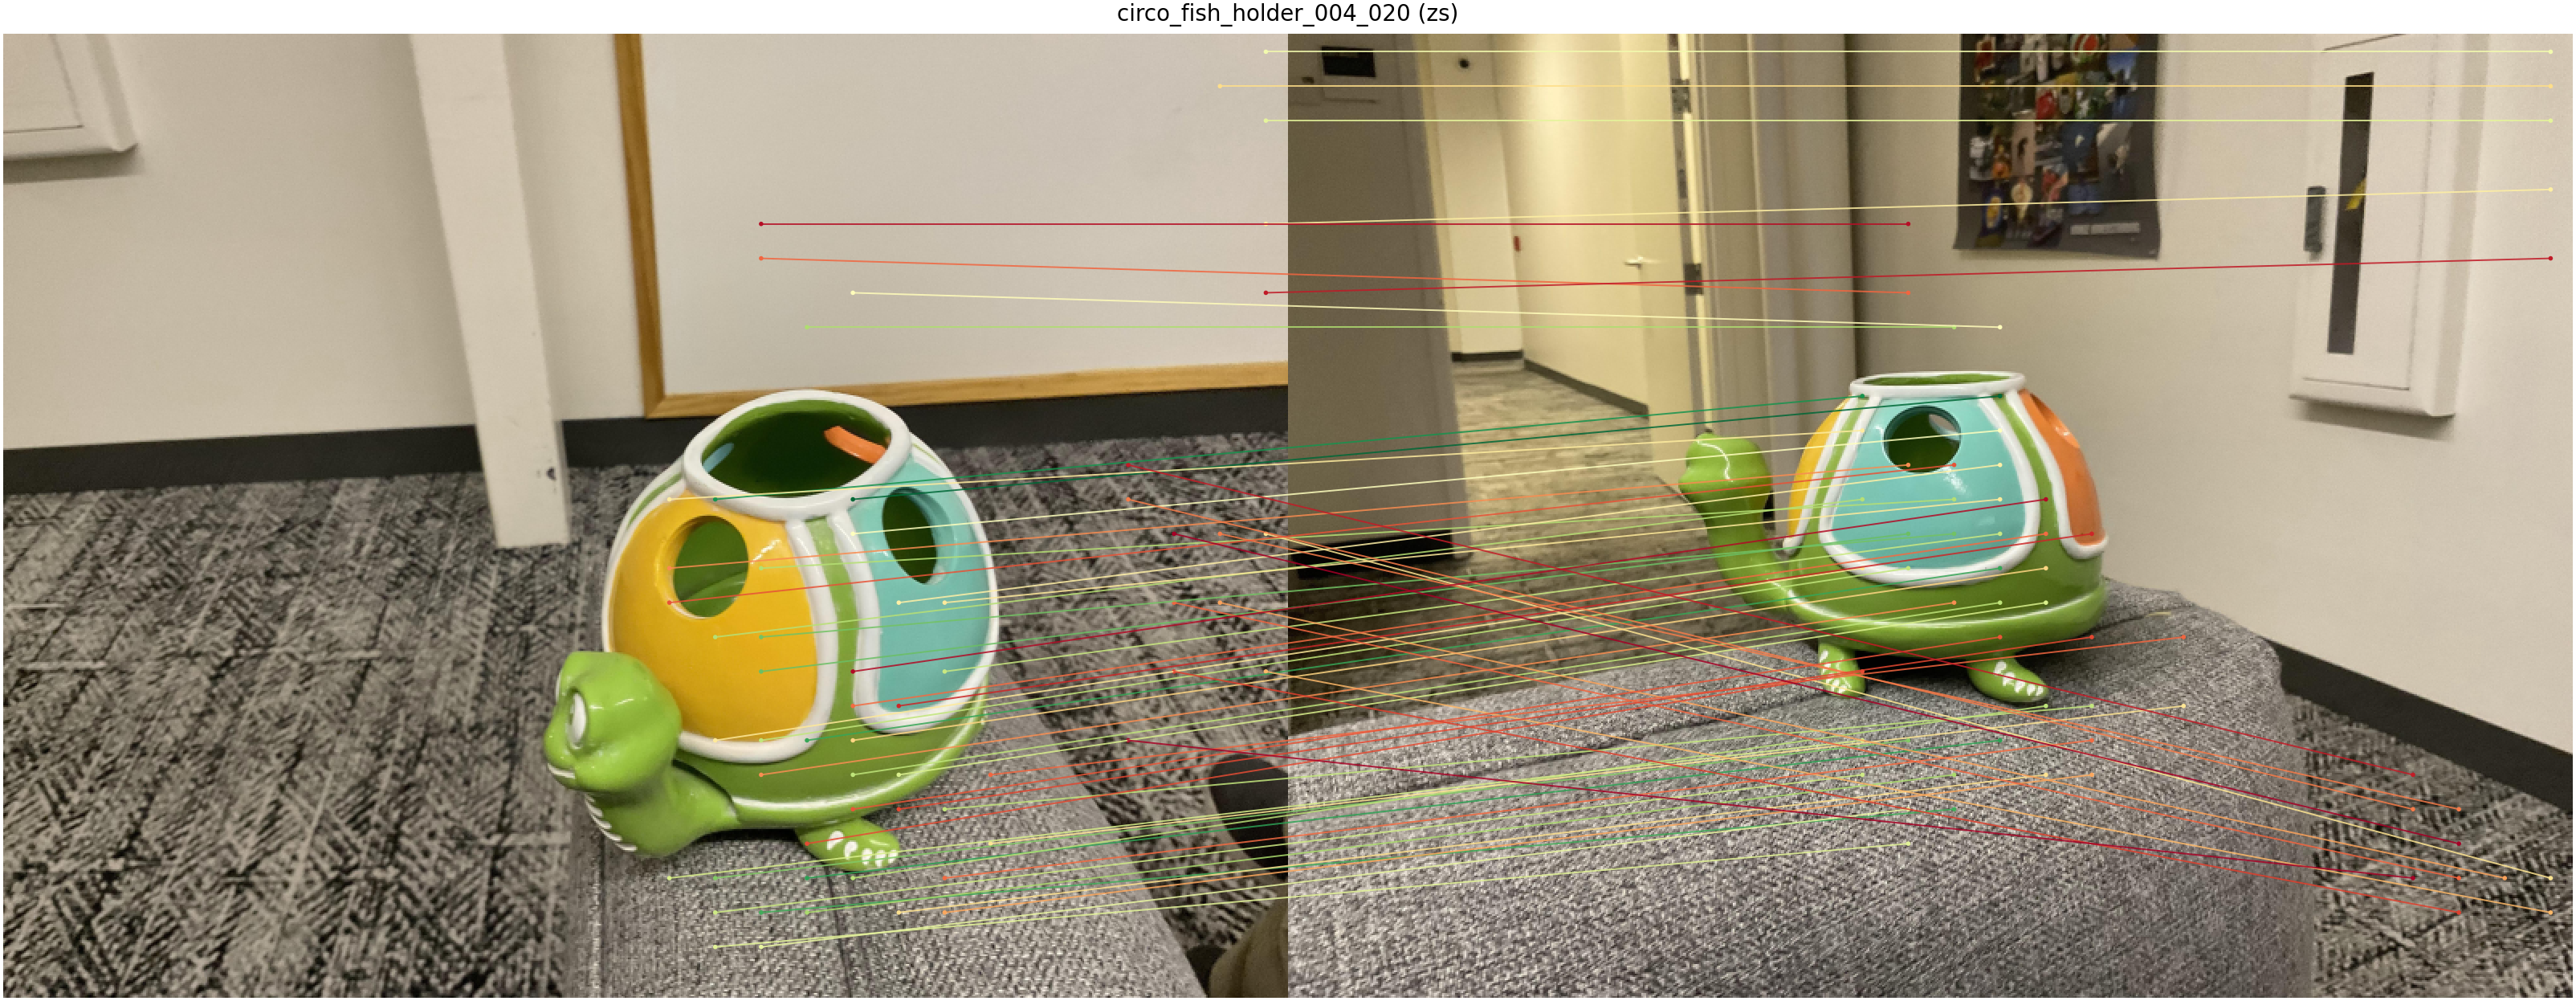
\includegraphics[width=\linewidth]{../teaser_pairs/teaser_zs_circo_fish_holder_004_020.png}
\caption{\textbf{The local feature matching task.} Two views of the
same object from a held-out NAVI scene; coloured lines are the top-60
mutual-nearest-neighbour patch correspondences produced by a
\emph{frozen, zero-shot} DINOv3 ViT-S/16 (no matching-specific
training), with green$=$high and red$=$low cosine similarity. Despite
strong viewpoint change, the foundation backbone already recovers a
largely geometry-consistent set of matches, motivating the question
studied in this paper: how much can a minimal, parameter-efficient
adaptation push this further?}
\label{fig:teaser}
\end{figure}

\paragraph{Contributions.}
\begin{itemize}
\item We reproduce on a foundation-model backbone the well-known
``LoRA + InfoNCE for matching'' recipe, with two modifications that
turn out to matter: (i) restricting LoRA to Q and V only and (ii)
combining HardInfoNCE with a 5-patch Safe-Radius mask
(Sec.~\ref{sec:method}).
\item We obtain consistent and reproducible NAVI matching gains across
two backbone sizes (Sec.~\ref{sec:results}).
\item We provide a multi-axis diagnostic analysis
(Sec.~\ref{sec:diag}) showing that the recipe leaves the underlying
representation essentially intact, and that gains under the strict
$5^\circ$ pose threshold do not materialize. We frame this honestly
as a limitation and discuss what kind of adapter or training data would
be needed to move the AUC@$5^\circ$ ceiling.
\end{itemize}

\section{Related Work}

\paragraph{Self-supervised vision foundation models.} The DINO line of
work~\cite{dino,dinov2,darcet2023registers} demonstrates that
self-supervised ViTs can learn dense patch features useful for tasks
ranging from segmentation to depth estimation, with no manual labels.
DINOv3 in particular is pre-trained on $\sim$170M images using DINO,
iBOT and register tokens~\cite{darcet2023registers}, and ships strong
zero-shot dense correspondence capability via simple cosine
nearest-neighbor matching. We adopt DINOv3 as a frozen backbone and ask
whether minimal adaptation can close the matching gap to specialised
detectors without disturbing the representation.

\paragraph{Parameter-efficient fine-tuning.} LoRA~\cite{lora}
parameterizes weight updates as a product of two low-rank matrices,
substantially reducing the number of trainable parameters. We use the
standard LoRA formulation with zero-initialized $B$ so that the
adapted model is identical to the frozen baseline at step~$0$, which is
particularly useful when the underlying foundation model already
produces strong features.

\paragraph{Local feature matching and camera pose.} A long line of
work, from hand-crafted detectors to learned matchers
(SuperPoint~\cite{superpoint}, SuperGlue~\cite{superglue},
LoFTR~\cite{loftr}, RoMa~\cite{roma}), targets matching directly. Our
contribution is orthogonal to these specialised matchers: rather than
designing a new matching architecture, we ask how far one can push
\emph{frozen} DINOv3 features as drop-in dense descriptors with only
a few hundred thousand trainable LoRA parameters.

\paragraph{Contrastive learning.} HardInfoNCE follows the InfoNCE
formulation~\cite{cpc,simclr} but, instead of using all in-batch
negatives, only retains the top-$K$ hardest. The Safe-Radius mask is
inspired by the observation that adjacent patches on the same physical
surface are positives in disguise; treating them as negatives directly
fights DINOv3's local smoothness prior.

\section{Method}
\label{sec:method}

The recipe is intentionally minimal so that each component can be
reasoned about independently. Below we describe (i) LoRA injection,
(ii) the HardInfoNCE + Safe-Radius loss, and (iii) the way ground-truth
positive correspondences are obtained from NAVI's depth maps.

\subsection{LoRA on Q and V}

For each transformer block, self-attention computes
$\text{softmax}(QK^\top / \sqrt{d_k}) V$ with
$Q = X W^Q$, $K = X W^K$, $V = X W^V$. We add LoRA adapters only to the
query and value projections:
\begin{equation}
W^Q \!\leftarrow\! W^Q + \tfrac{\alpha}{r} B^Q A^Q,\quad
W^V \!\leftarrow\! W^V + \tfrac{\alpha}{r} B^V A^V,
\end{equation}
with $A \in \mathbb{R}^{r\times d}$ Kaiming-initialized,
$B \in \mathbb{R}^{d\times r}$ zero-initialized,
$r=4$, $\alpha=8$. All other parameters of DINOv3 (including
$W^K, W^O$, FFN, layer-norms, register tokens, the patch embedding
and the 2D-RoPE positional code) are frozen. Because $B=0$ at
initialization, $\Delta W = 0$ and the LoRA model reproduces the
zero-shot DINOv3 output exactly at step~$0$; gradient flow can only
\emph{add} information rather than first having to recover what was
already there.

We choose Q+V (rather than Q+K, all of Q/K/V/O, or attaching adapters
to the FFN as well) for two reasons. First, perturbing $W^K$ directly
distorts the attention pattern that drives DINOv3's pre-trained
clustering behavior. Second, restricting the adapter to two
projections per block keeps the trainable parameter count well below
$1\%$ of the backbone, which empirically prevents the recipe from
degenerating into a feature replacement on a small contrastive corpus.

\subsection{HardInfoNCE with Safe Radius}

For an anchor patch $a$ and its ground-truth positive $p$, let $s_i^+ =
\cos(\hat f_a, \hat f_p)$ where $\hat f$ denotes the L2-normalized
patch embedding. Negatives are drawn from the union of (i) all other
patches in the anchor's own image and (ii) all patches of the
remaining 7 images in the mini-batch (true cross-scene negatives). For
each anchor we then keep only the top-$K=128$ negatives ranked by
similarity:
\begin{equation}
\mathcal{L}_a = -\log\frac{\exp(s_a^+/\tau)}{\exp(s_a^+/\tau) +
\sum_{j\in\mathrm{HardK}(a)} \exp(s_j^-/\tau)},
\end{equation}
with $\tau = 0.07$.

The cross-scene component is critical: had we drawn $K$ negatives only
from the anchor's own image, the loss would reduce to enforcing
intra-image distinguishability and quickly hit the
$\ln(K\!+\!1)$ trivial floor. Conversely, naive in-image negatives
contain many that are spatially adjacent to $a$ and therefore lie on
the same physical surface; treating them as negatives forces the model
to push adjacent patches apart and disrupts DINOv3's local smoothness
prior. We address this with a \textbf{Safe Radius}: any in-image
patch whose 2D coordinate on the patch grid is within
L$_\infty$-distance 5 of the anchor is removed from the negative pool.
The mask is computed once per image and is independent of the random
training pair.

\subsection{Ground-truth correspondences from NAVI}

Given a training pair $(A, B)$ with depth maps $D_A, D_B$, intrinsics
$K_A, K_B$ and relative pose $T_{A\to B}$, every patch centre in $A$
is back-projected to 3D using $D_A$ and re-projected into image
$B$. The symmetric procedure is then applied for $B\to A$. A
patch pair is retained as a ground-truth positive when both directions
agree within a fixed pixel threshold; all other patches are eligible
negatives. This procedure yields a clean set of patch-level positives
without any hand-tuned scoring.

\subsection{Training recipe}
We use AdamW with learning rate $1\!\times\!10^{-4}$, weight decay
$1\!\times\!10^{-4}$ and a cosine schedule for 15 epochs. Mini-batch
size is $8$ pairs. Checkpoints are saved every 3 epochs and evaluated
on the full held-out NAVI test split (Sec.~\ref{sec:setup}); the best
epoch is selected by test-set Precision. End-to-end wall-clock is
$\sim$5.5h for ViT-S/16 and $\sim$11h for ViT-L/16 on a single
NVIDIA A100 GPU.

\section{Experiments}
\label{sec:results}

\subsection{Dataset and protocol}
\label{sec:setup}

\paragraph{Split.} NAVI v1.5 ships no per-image split labels; we
adopt a deterministic \emph{scene-level} split with seed
\texttt{12345}: the list of \texttt{multiview\_*} scenes is shuffled
and the last $15\%$ are reserved as the held-out test partition.
Because every image of a given scene goes entirely to one side, the
resulting split is image- and scene-disjoint by construction
(Tab.~\ref{tab:split}), removing the most common single-object
evaluation leakage.

\paragraph{Pairs.} For each scene we enumerate all view pairs and
retain only those with relative camera rotation in
$[10^\circ, 90^\circ]$, then cap at 20 train / 12 test pairs per
scene. The result is $5\,596$ training and $908$ test pairs.

\paragraph{Image geometry.} All images are resized so that the longer
side equals $1024$. With patch size $16$, this yields a $64\times64$
patch grid for evaluation.

\paragraph{Pose-evaluation pipeline.} Following the SuperGlue
protocol~\cite{superglue} we (i) extract patch features, (ii) form
mutual-nearest-neighbor matches in feature space, (iii) estimate the
Essential matrix via USAC~\cite{usac}, (iv) decompose into $(R,t)$ via
SVD and the cheirality check~\cite{nister2004}, and (v) compute the
angular pose error against ground truth. We report
AUC@$5^\circ\!/10^\circ\!/20^\circ$ and Precision: the fraction of
MNN matches whose Sampson distance under the ground-truth
Essential matrix is below $5\!\times\!10^{-4}$ in $1024^2$
coordinates. The same pipeline is applied to zero-shot DINOv3 and to
each LoRA checkpoint, so all reported gains are recipe-attributable.

\begin{table}[t]
\centering\small
\caption{Scene-disjoint NAVI split used throughout the paper.
Train and test partitions share no images by construction.}
\label{tab:split}
\begin{tabular}{@{}lccc@{}}
\toprule
\textbf{Split} & \textbf{Scenes} & \textbf{Pairs} & \textbf{Cap / scene}\\
\midrule
Train & $\sim$275 (85\%) & 5\,596 & 20 \\
Test  & $\sim$49\,(15\%) & 908   & 12 \\
\bottomrule
\end{tabular}
\end{table}

\subsection{Per-epoch dynamics}

Fig.~\ref{fig:per_epoch} plots Precision, AUC@$10^\circ$ and
AUC@$20^\circ$ at every saved epoch for both backbones, together with
the corresponding zero-shot baselines (dashed). Both backbones cross
above the zero-shot Precision baseline by epoch~$2$--$3$ and
stabilize around $+7$ pp; AUC@$20^\circ$ grows by roughly $2\times$
the zero-shot value. Curves are monotonically non-decreasing in
Precision, indicating that the recipe is robust to the exact
choice of stopping epoch.

\begin{figure*}[t]
\centering
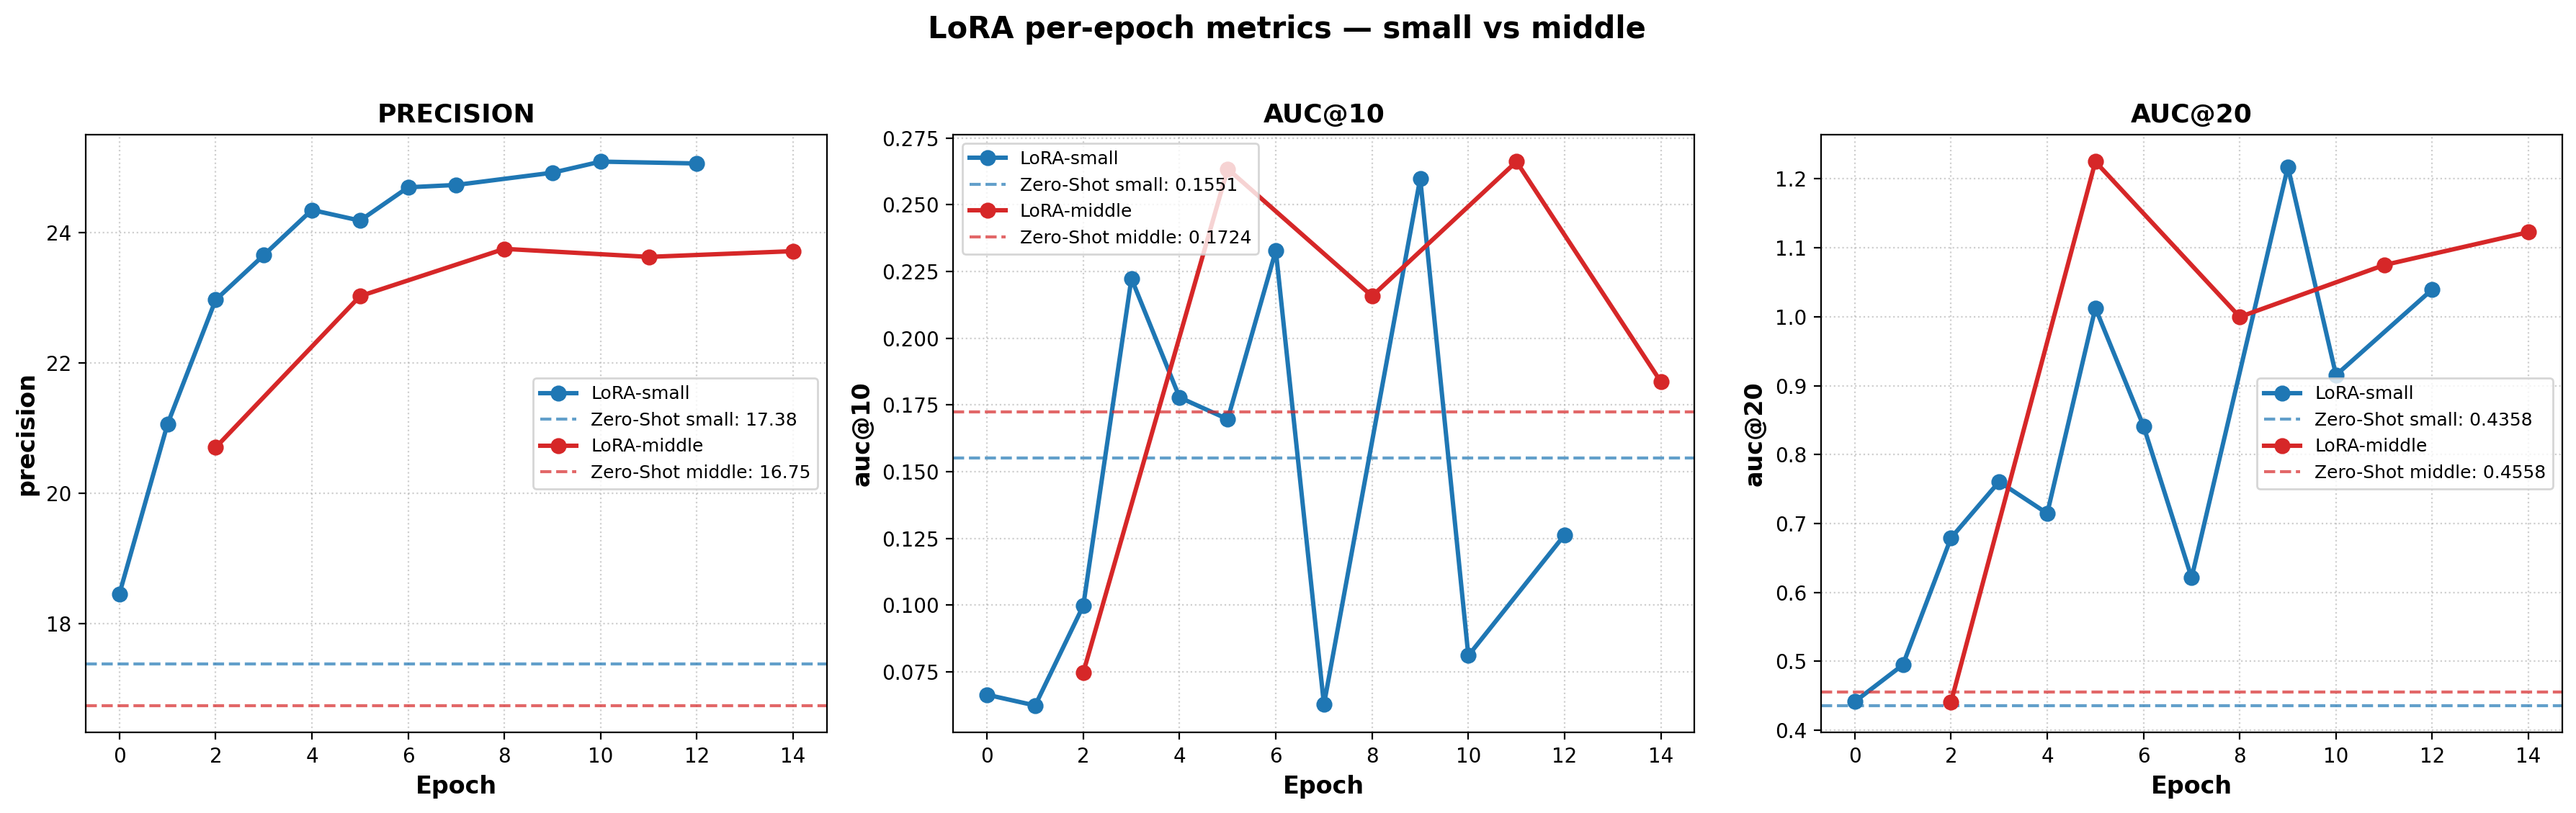
\includegraphics[width=0.97\linewidth]{../presentation/result/per_epoch_small_vs_middle.png}
\caption{Per-epoch metrics on NAVI for ViT-S/16 (left) and ViT-L/16
(right). Solid: LoRA-tuned; dashed: zero-shot baseline. Both backbones
cross above the zero-shot Precision baseline by epoch~3 and stabilize
around $+7$ pp.}
\label{fig:per_epoch}
\end{figure*}

\subsection{Final numerical results}

Tab.~\ref{tab:final} reports the best-epoch numbers for each
backbone against its own zero-shot baseline. The best epoch is
selected by highest test-set Precision among saved checkpoints.

\begin{table}[t]
\centering\small
\caption{NAVI test (908 pairs, $1024^2$ evaluation). LoRA + Safe
Radius improves Precision and AUC@$20^\circ$ on both backbones.
AUC@$5^\circ$ stays flat or drops, which we discuss in
Sec.~\ref{sec:limits}.}
\label{tab:final}
\setlength{\tabcolsep}{4pt}
\begin{tabular}{@{}llcccc@{}}
\toprule
\textbf{Backbone} & \textbf{Setting} & \textbf{AUC@5} & \textbf{AUC@10} & \textbf{AUC@20} & \textbf{Prec.}\\
\midrule
\multirow{2}{*}{ViT-S/16}
  & Zero-shot                       & 0.076 & 0.155 & 0.436 & 17.38\%\\
  & LoRA (ep.~12)                   & 0.000 & 0.126 & 1.040 & \textbf{25.06\%}\\
\midrule
\multirow{2}{*}{ViT-L/16}
  & Zero-shot                       & 0.059 & 0.172 & 0.456 & 16.75\%\\
  & LoRA (ep.~14)                   & 0.061 & 0.184 & 1.123 & \textbf{23.71\%}\\
\bottomrule
\end{tabular}
\end{table}

The gains on Precision and AUC@$20^\circ$ are unambiguous and
consistent across the two backbone sizes. At the strict $5^\circ$
threshold, however, AUC@$5^\circ$ \emph{drops} on ViT-S/16
($0.076\!\to\!0.000$) and is essentially unchanged on ViT-L/16
($0.059\!\to\!0.061$). The recipe therefore adds many
``borderline-correct'' matches that the wide threshold counts as
successes, but does not produce more high-precision pose recoveries
at the strict end. We treat this as a real limitation and return to
it in Sec.~\ref{sec:limits}.

\subsection{Diagnostic analysis: how much did the features actually move?}
\label{sec:diag}

To understand whether the LoRA update reshapes the feature space or
merely tilts it, we compare zero-shot and LoRA features on a fixed
30-image NAVI subset.

\paragraph{Aggregate diagnostics.} Fig.~\ref{fig:bars} aggregates six
representation diagnostics into bar charts: mean intra-image cosine
(lower~$=$~more distinguishable patches), positive-pair cosine (higher
$=$ better aligned positives), effective rank (numerical rank of the
patch-token covariance), neighbourhood dominance (how often the
nearest neighbour of a patch lies within the same image), and PCA
basis stability. Across all of them the LoRA bar is within a few
percent of the zero-shot bar; effective rank and neighbourhood
dominance change by $\le 0.002$ in absolute terms.

\begin{figure}[t]
\centering
\begin{subfigure}{0.49\linewidth}
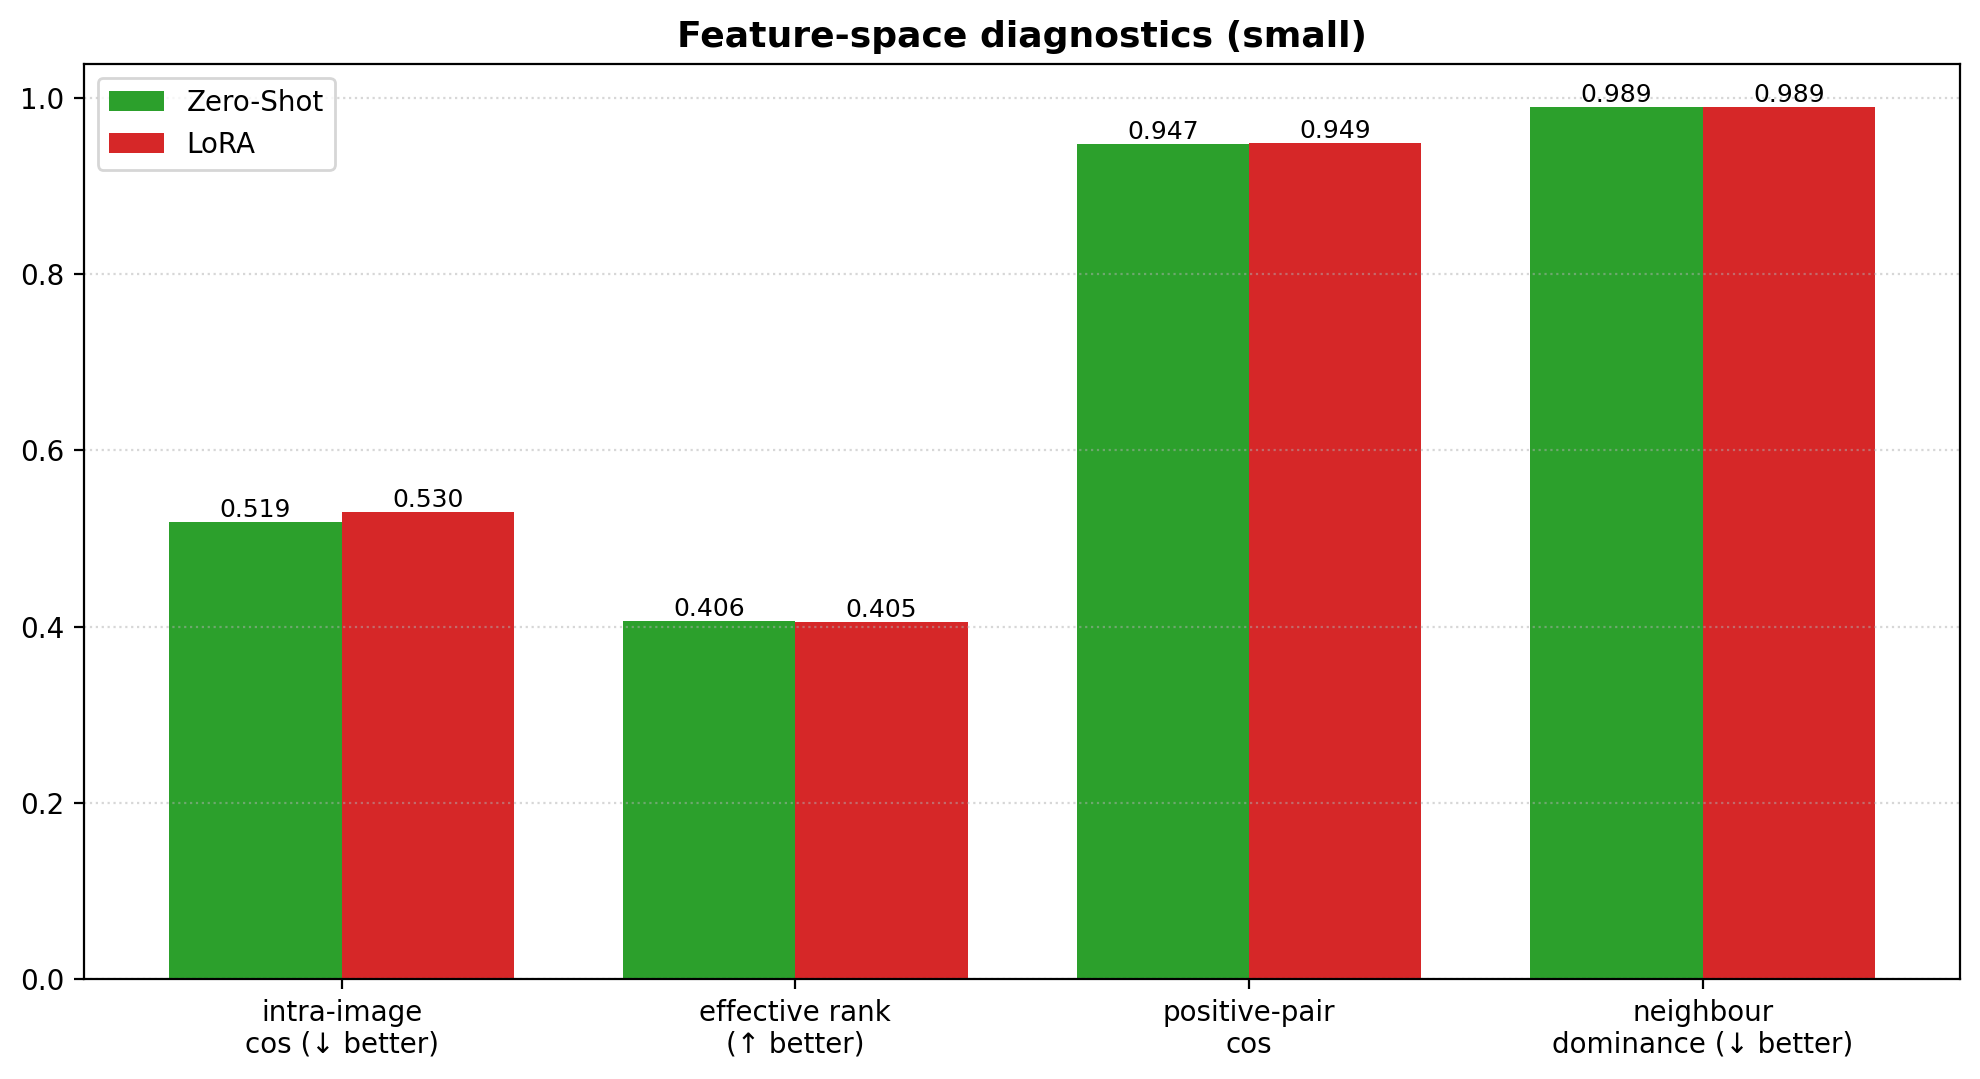
\includegraphics[width=\linewidth]{../presentation/result/diag_small/bars_summary_small.png}
\caption{ViT-S/16}
\end{subfigure}\hfill
\begin{subfigure}{0.49\linewidth}
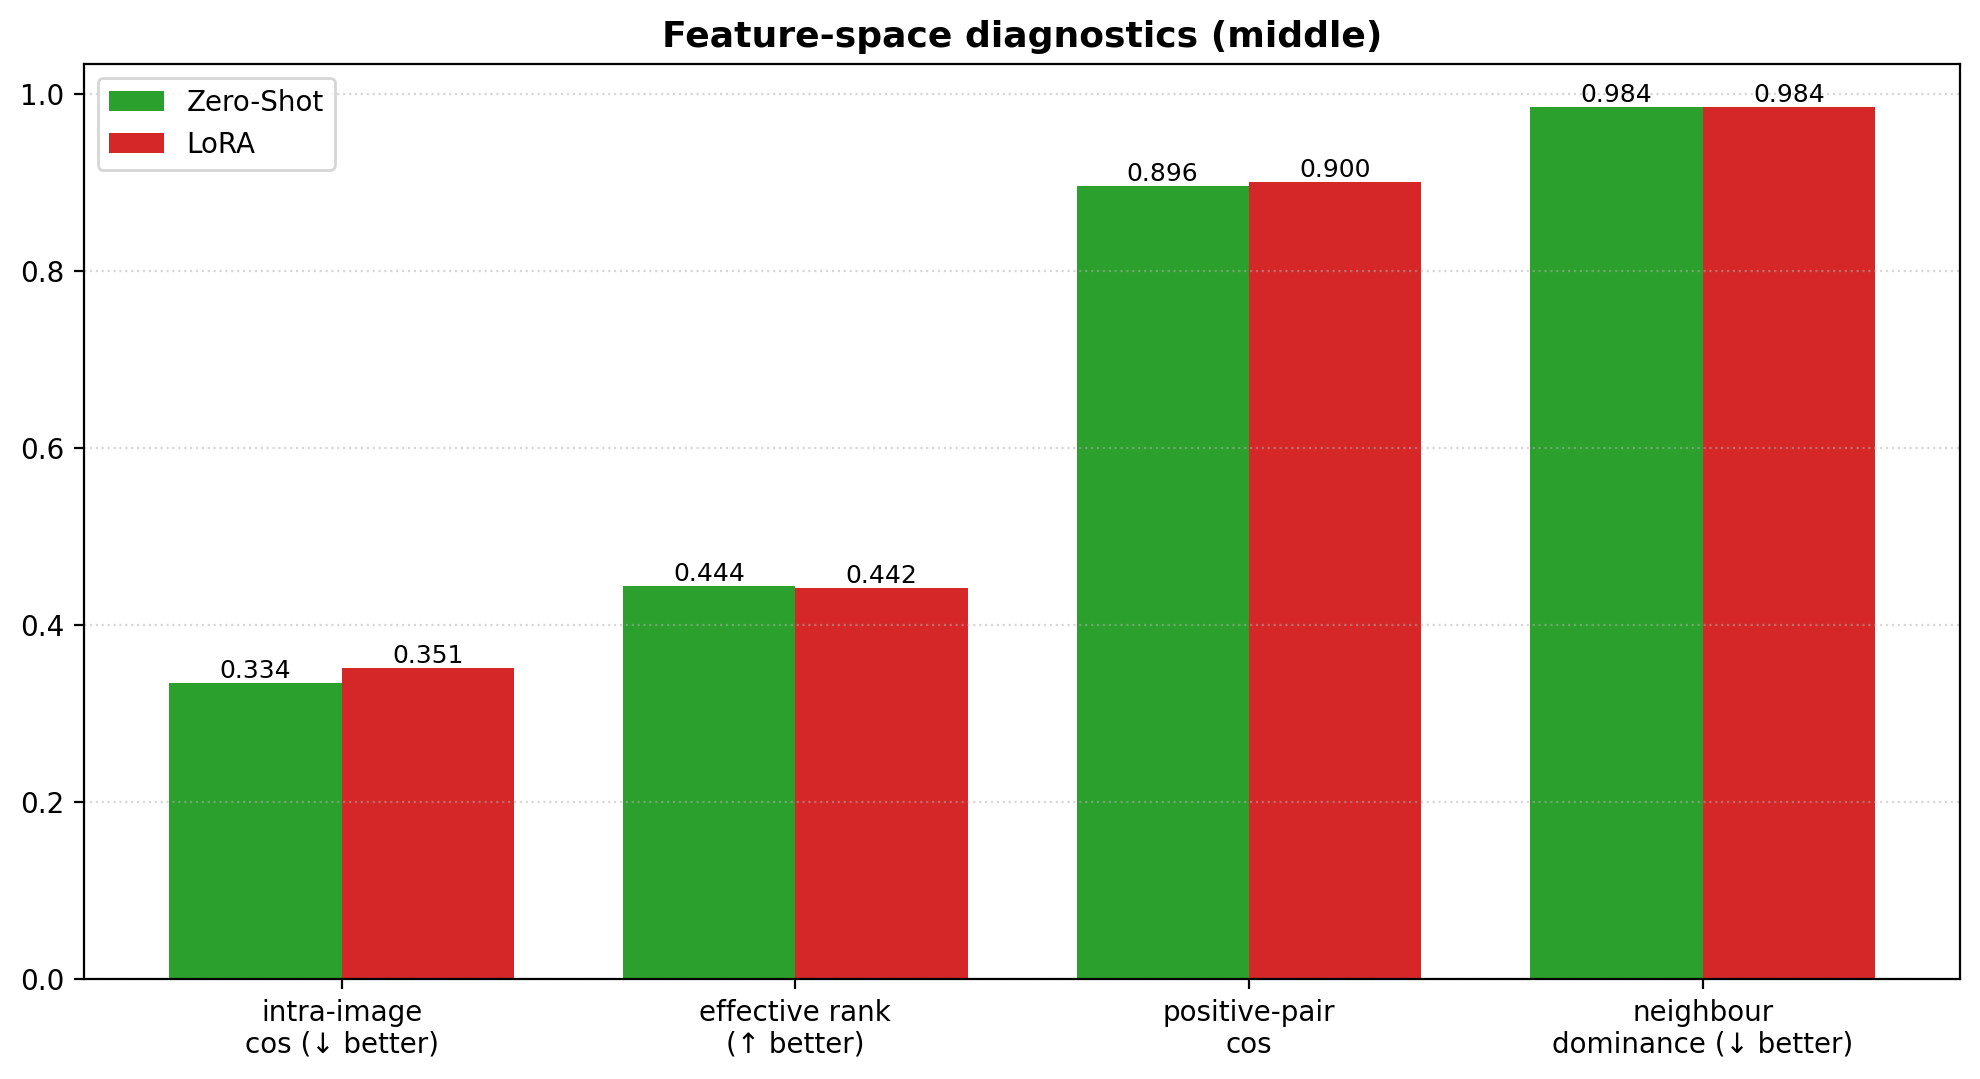
\includegraphics[width=\linewidth]{../presentation/result/diag_middle/bars_summary_middle.png}
\caption{ViT-L/16}
\end{subfigure}
\caption{Aggregate representation-level diagnostics on a 30-image NAVI
subset. All metrics move by $\le 0.02$ in absolute terms; the
dominant signal of LoRA is \emph{not} a redrawn feature space.}
\label{fig:bars}
\end{figure}

\paragraph{Per-image distinguishability.} Per-image mean intra-image
patch cosine (Fig.~\ref{fig:hist_intra}) shifts only marginally to
the right under LoRA on both backbones, indicating LoRA features are
in fact \emph{slightly less} distinguishable than zero-shot ones at
the patch level (S/16: $+0.011$, L/16: $+0.017$). Positive-pair
cosine (Fig.~\ref{fig:hist_pos}) is already saturated under zero-shot
DINOv3 ($\sim\!0.95$ on S/16, $\sim\!0.90$ on L/16) and the LoRA
fine-tune moves the mean by $\le 0.005$. Whatever gain we observe on
NAVI must therefore come from \emph{relative} re-ranking rather than
from absolute alignment improvement.

\begin{figure}[t]
\centering
\begin{subfigure}{0.49\linewidth}
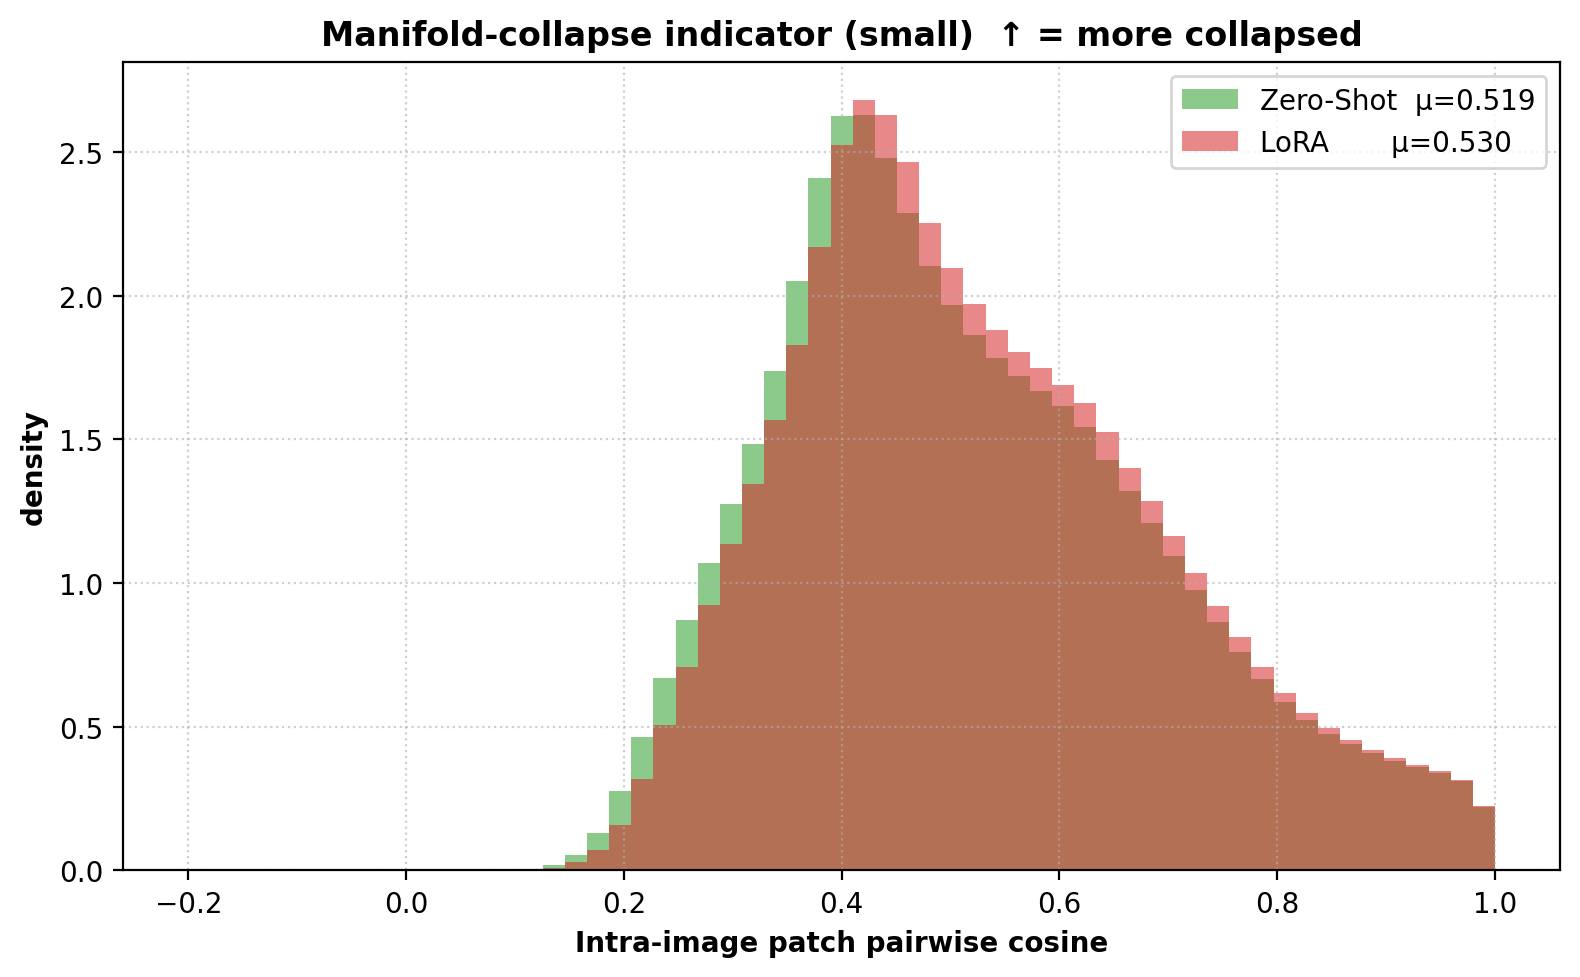
\includegraphics[width=\linewidth]{../presentation/result/diag_small/hist_intra_cos_small.png}
\caption{Intra-cos, S/16}
\end{subfigure}\hfill
\begin{subfigure}{0.49\linewidth}
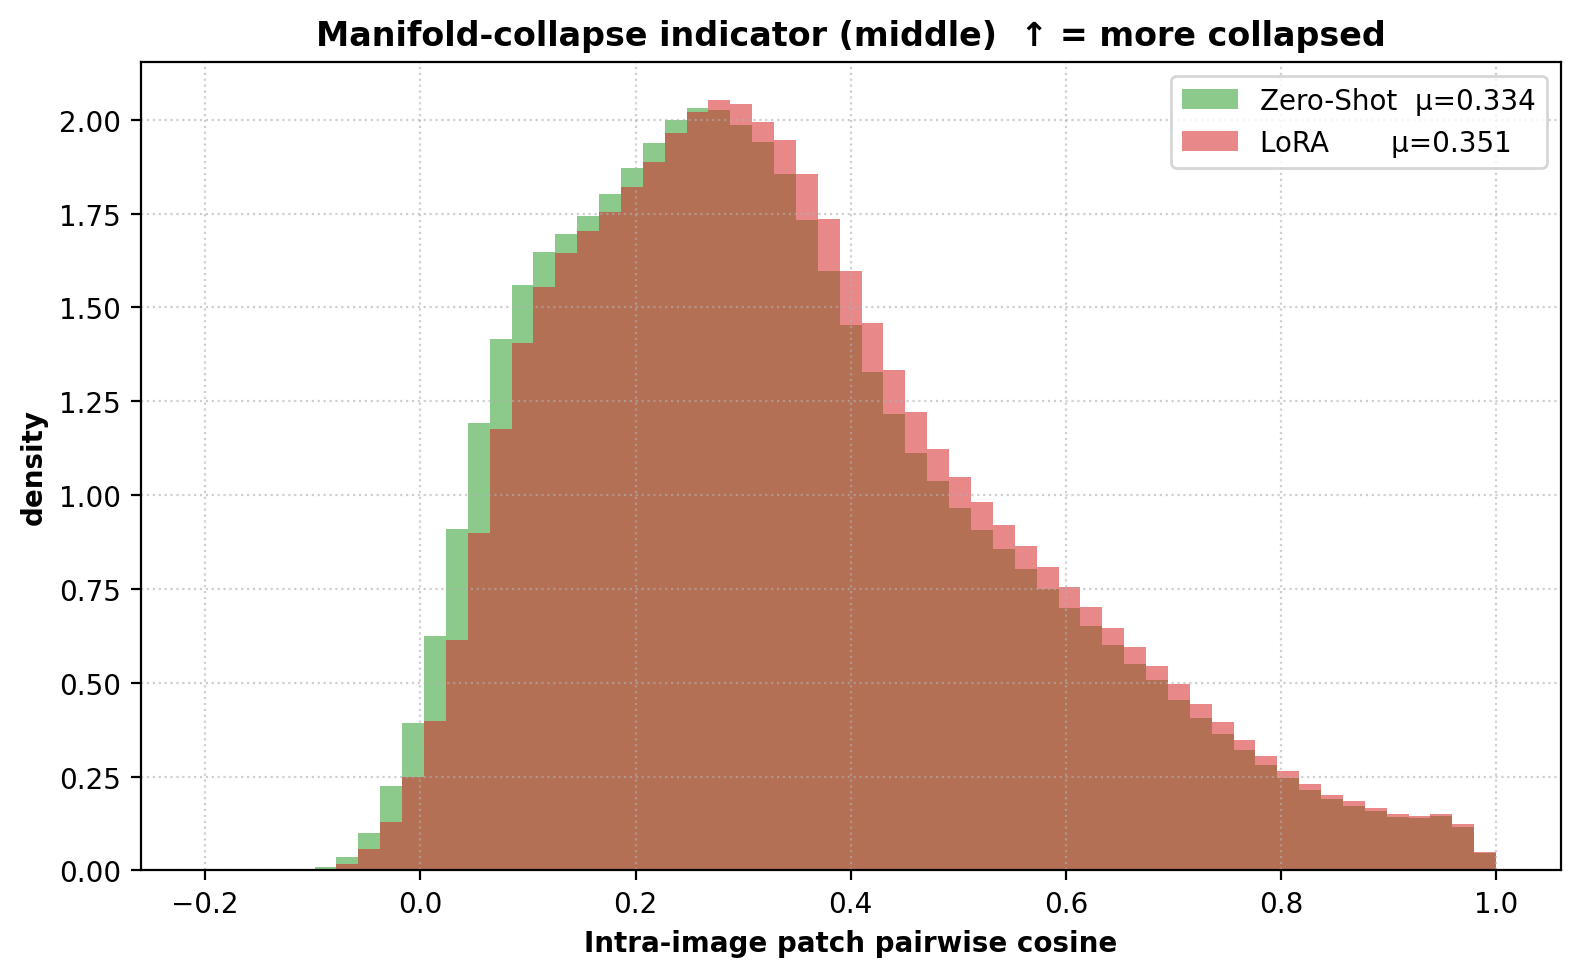
\includegraphics[width=\linewidth]{../presentation/result/diag_middle/hist_intra_cos_middle.png}
\caption{Intra-cos, L/16}
\end{subfigure}
\caption{Distribution of per-image mean intra-image patch cosine.
LoRA shifts the histogram only slightly to the right.}
\label{fig:hist_intra}
\end{figure}

\begin{figure}[t]
\centering
\begin{subfigure}{0.49\linewidth}
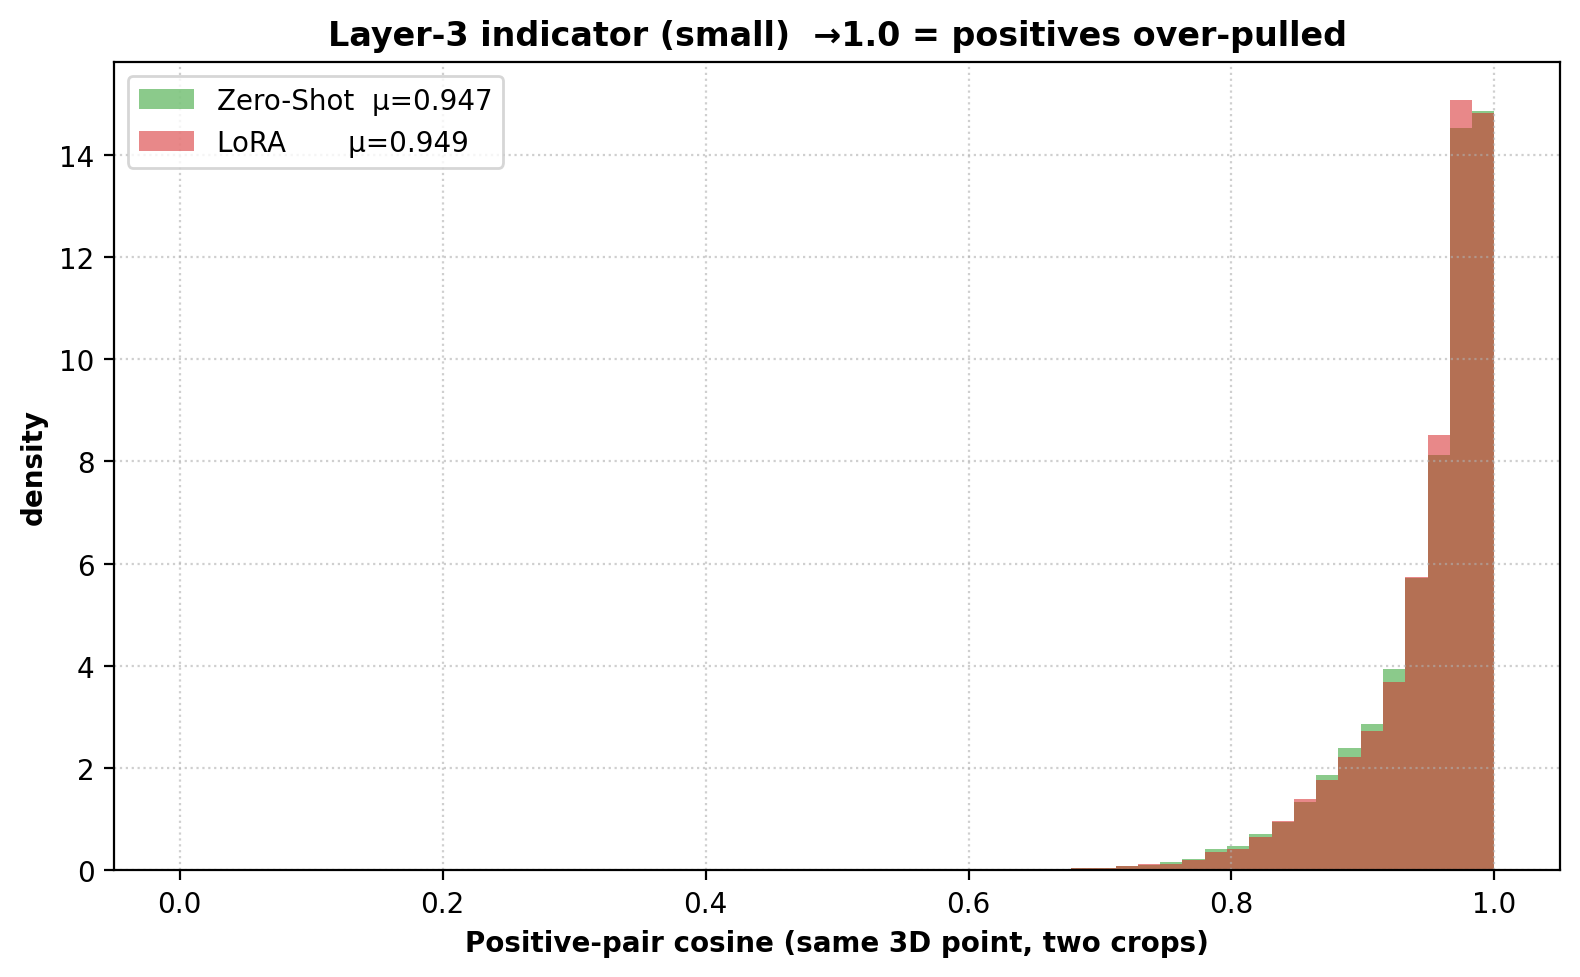
\includegraphics[width=\linewidth]{../presentation/result/diag_small/hist_pos_cos_small.png}
\caption{Pos-cos, S/16}
\end{subfigure}\hfill
\begin{subfigure}{0.49\linewidth}
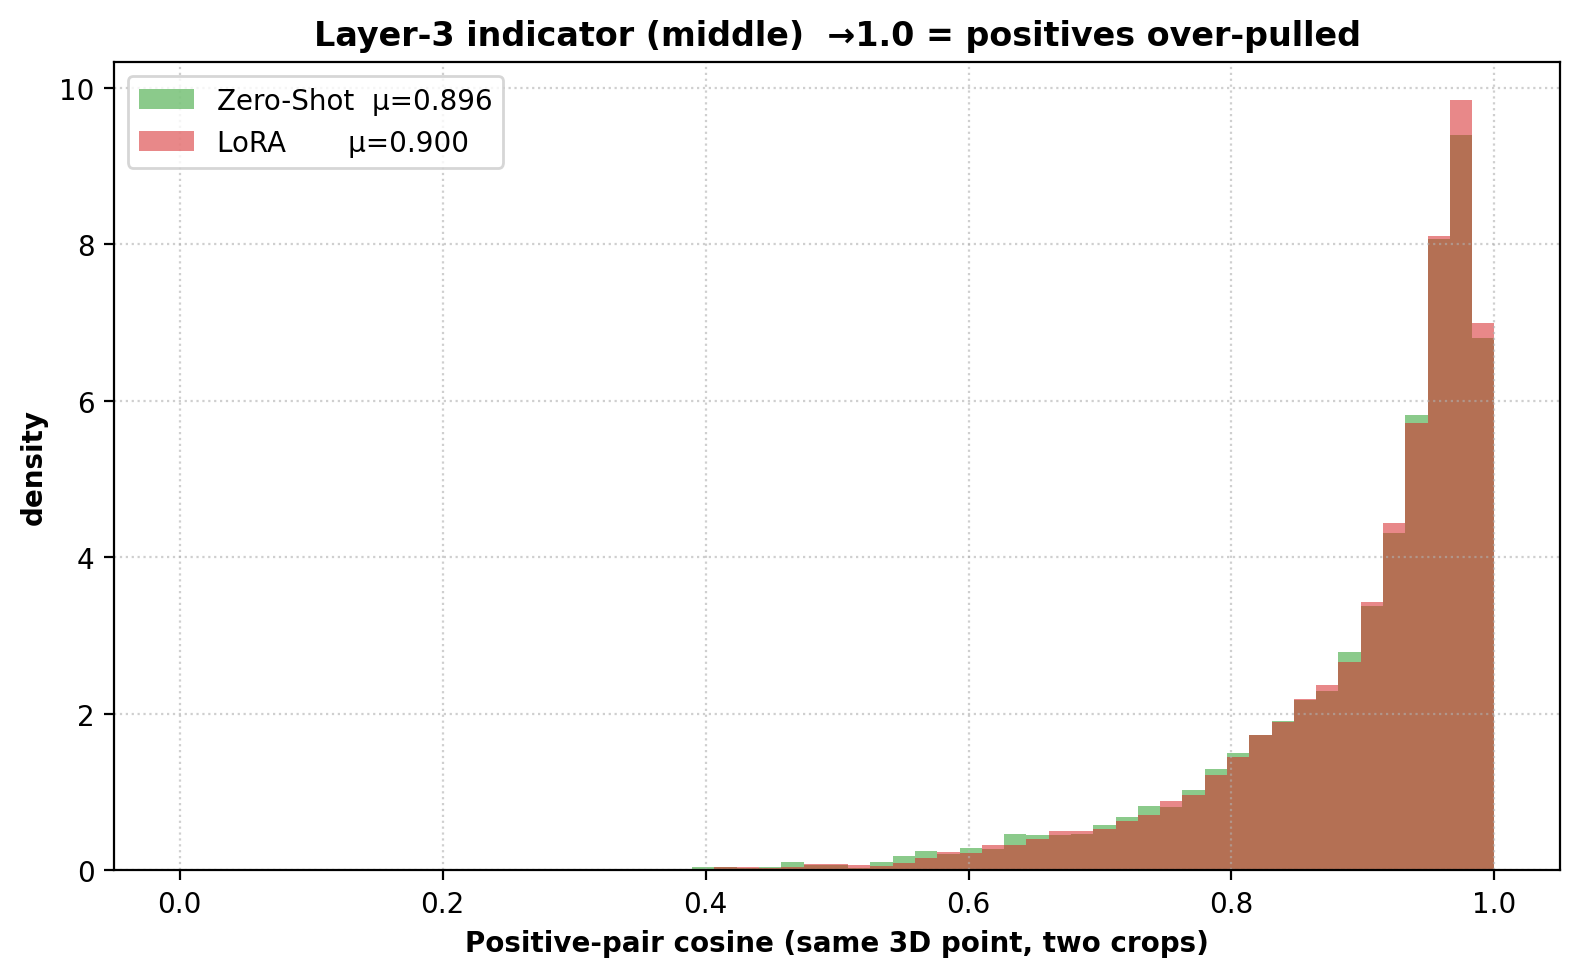
\includegraphics[width=\linewidth]{../presentation/result/diag_middle/hist_pos_cos_middle.png}
\caption{Pos-cos, L/16}
\end{subfigure}
\caption{Cosine similarity of ground-truth positive patch pairs.
The two histograms are nearly indistinguishable.}
\label{fig:hist_pos}
\end{figure}

\paragraph{Qualitative PCA visualization.}
Fig.~\ref{fig:pca} projects the patch tokens of a single NAVI image
to RGB via PCA, comparing zero-shot DINOv3 (top row) with the LoRA
fine-tuned model (bottom row) on both backbones. The four panels are
visually nearly identical: same object boundaries, same coarse-to-fine
colour gradients, same background blob. Whatever LoRA changed is
below the resolution of a 3-channel PCA visualization, and is
consistent across the two model sizes.

\begin{figure}[t]
\centering
\begin{subfigure}{0.49\linewidth}
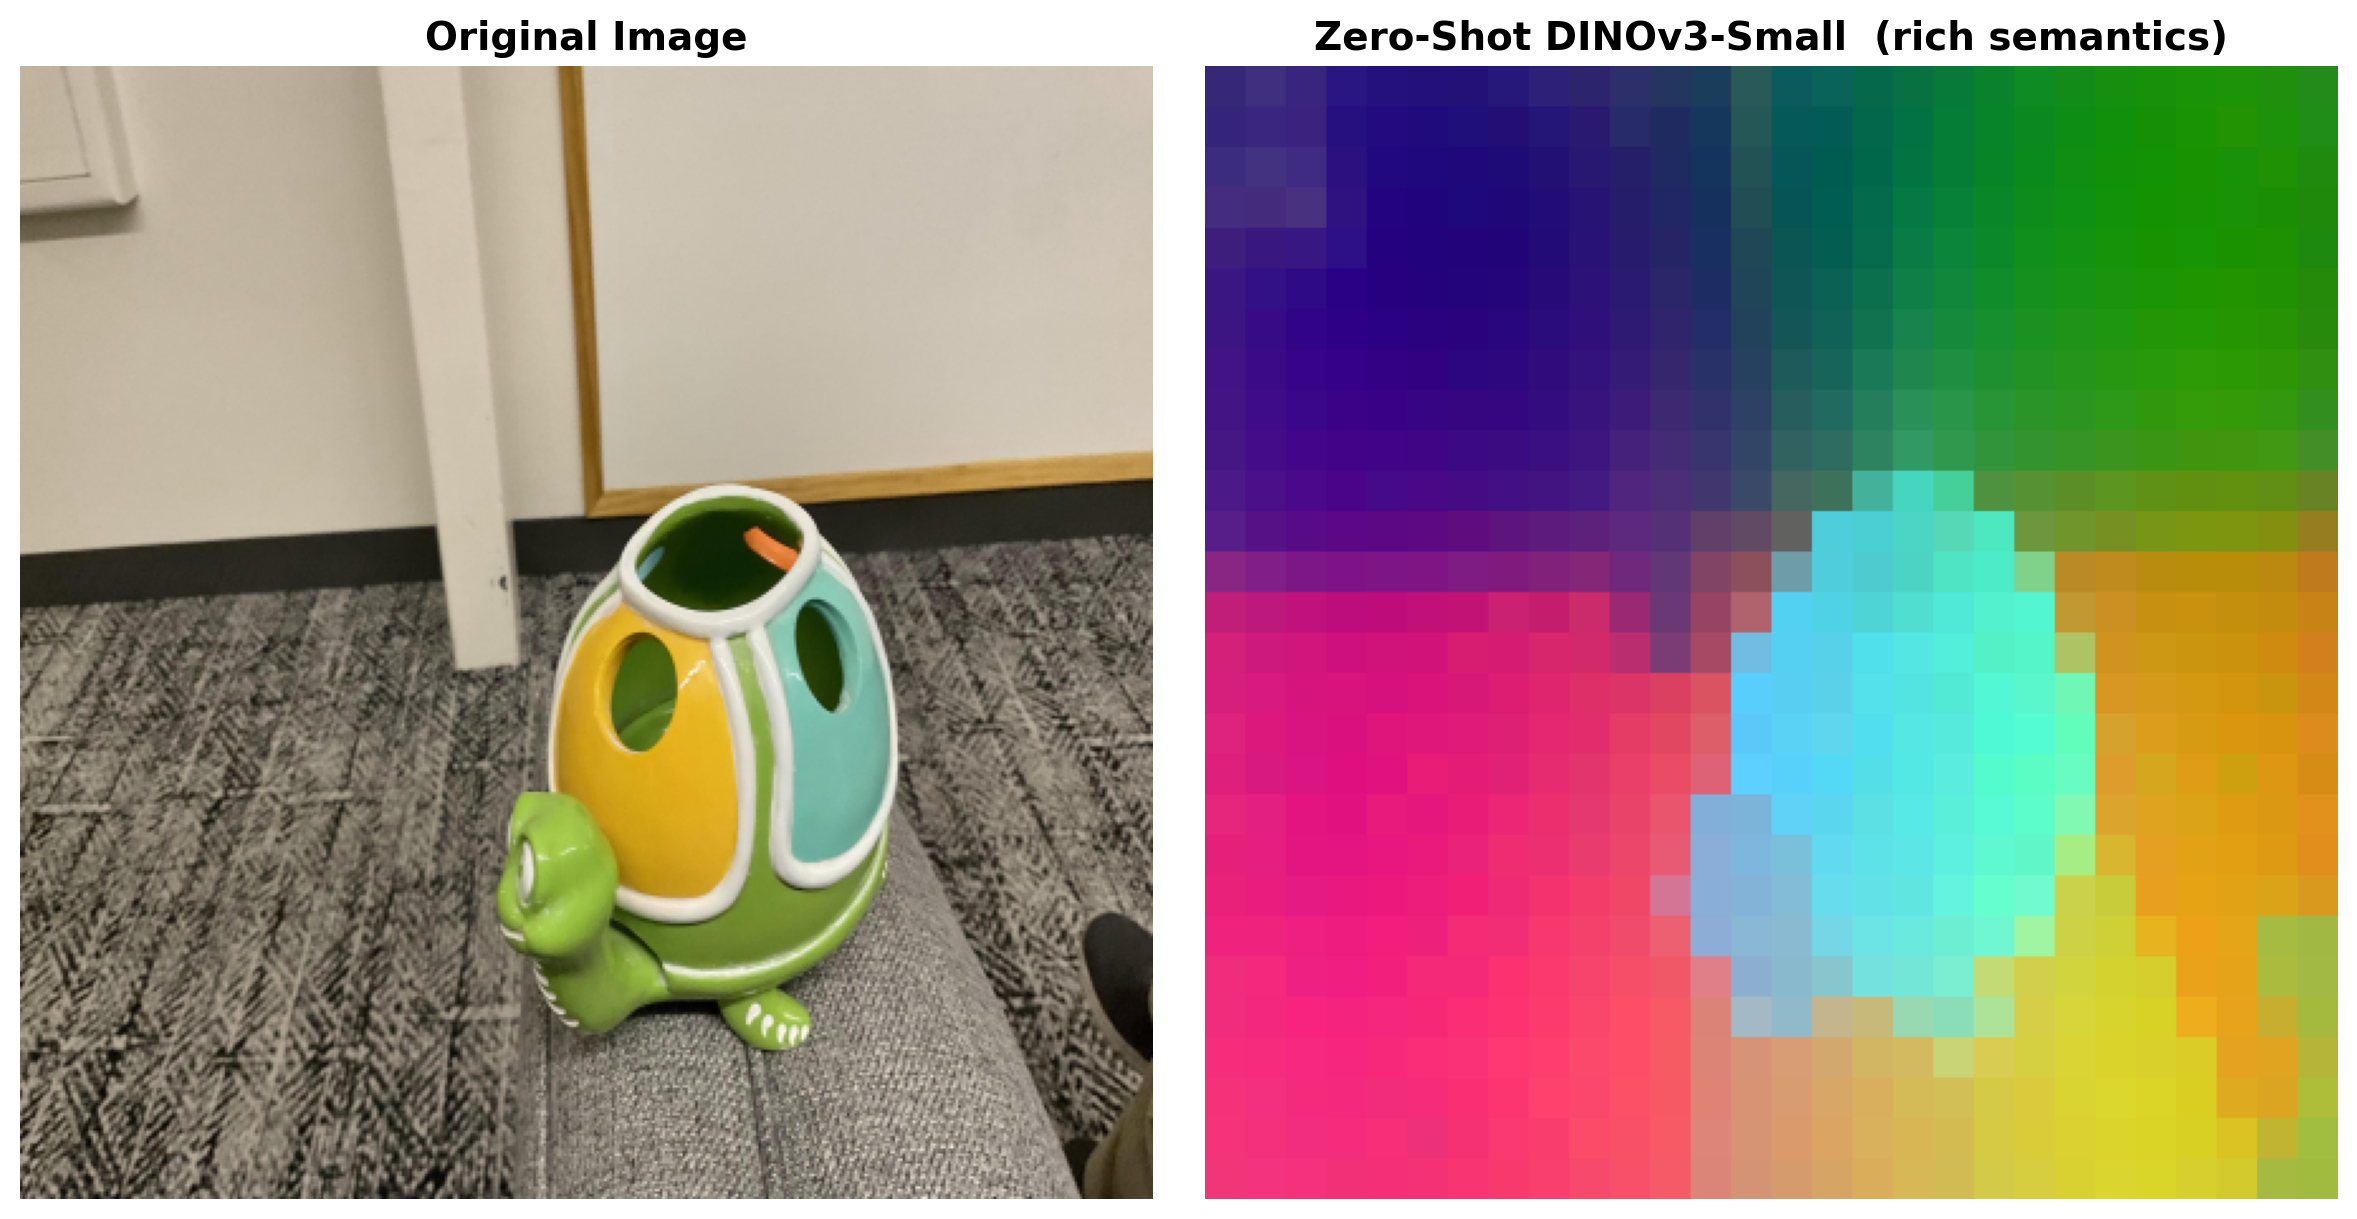
\includegraphics[width=\linewidth]{../presentation/result/diag_small/pca_small_004_zs.png}
\caption{ViT-S/16: zero-shot}
\end{subfigure}\hfill
\begin{subfigure}{0.49\linewidth}
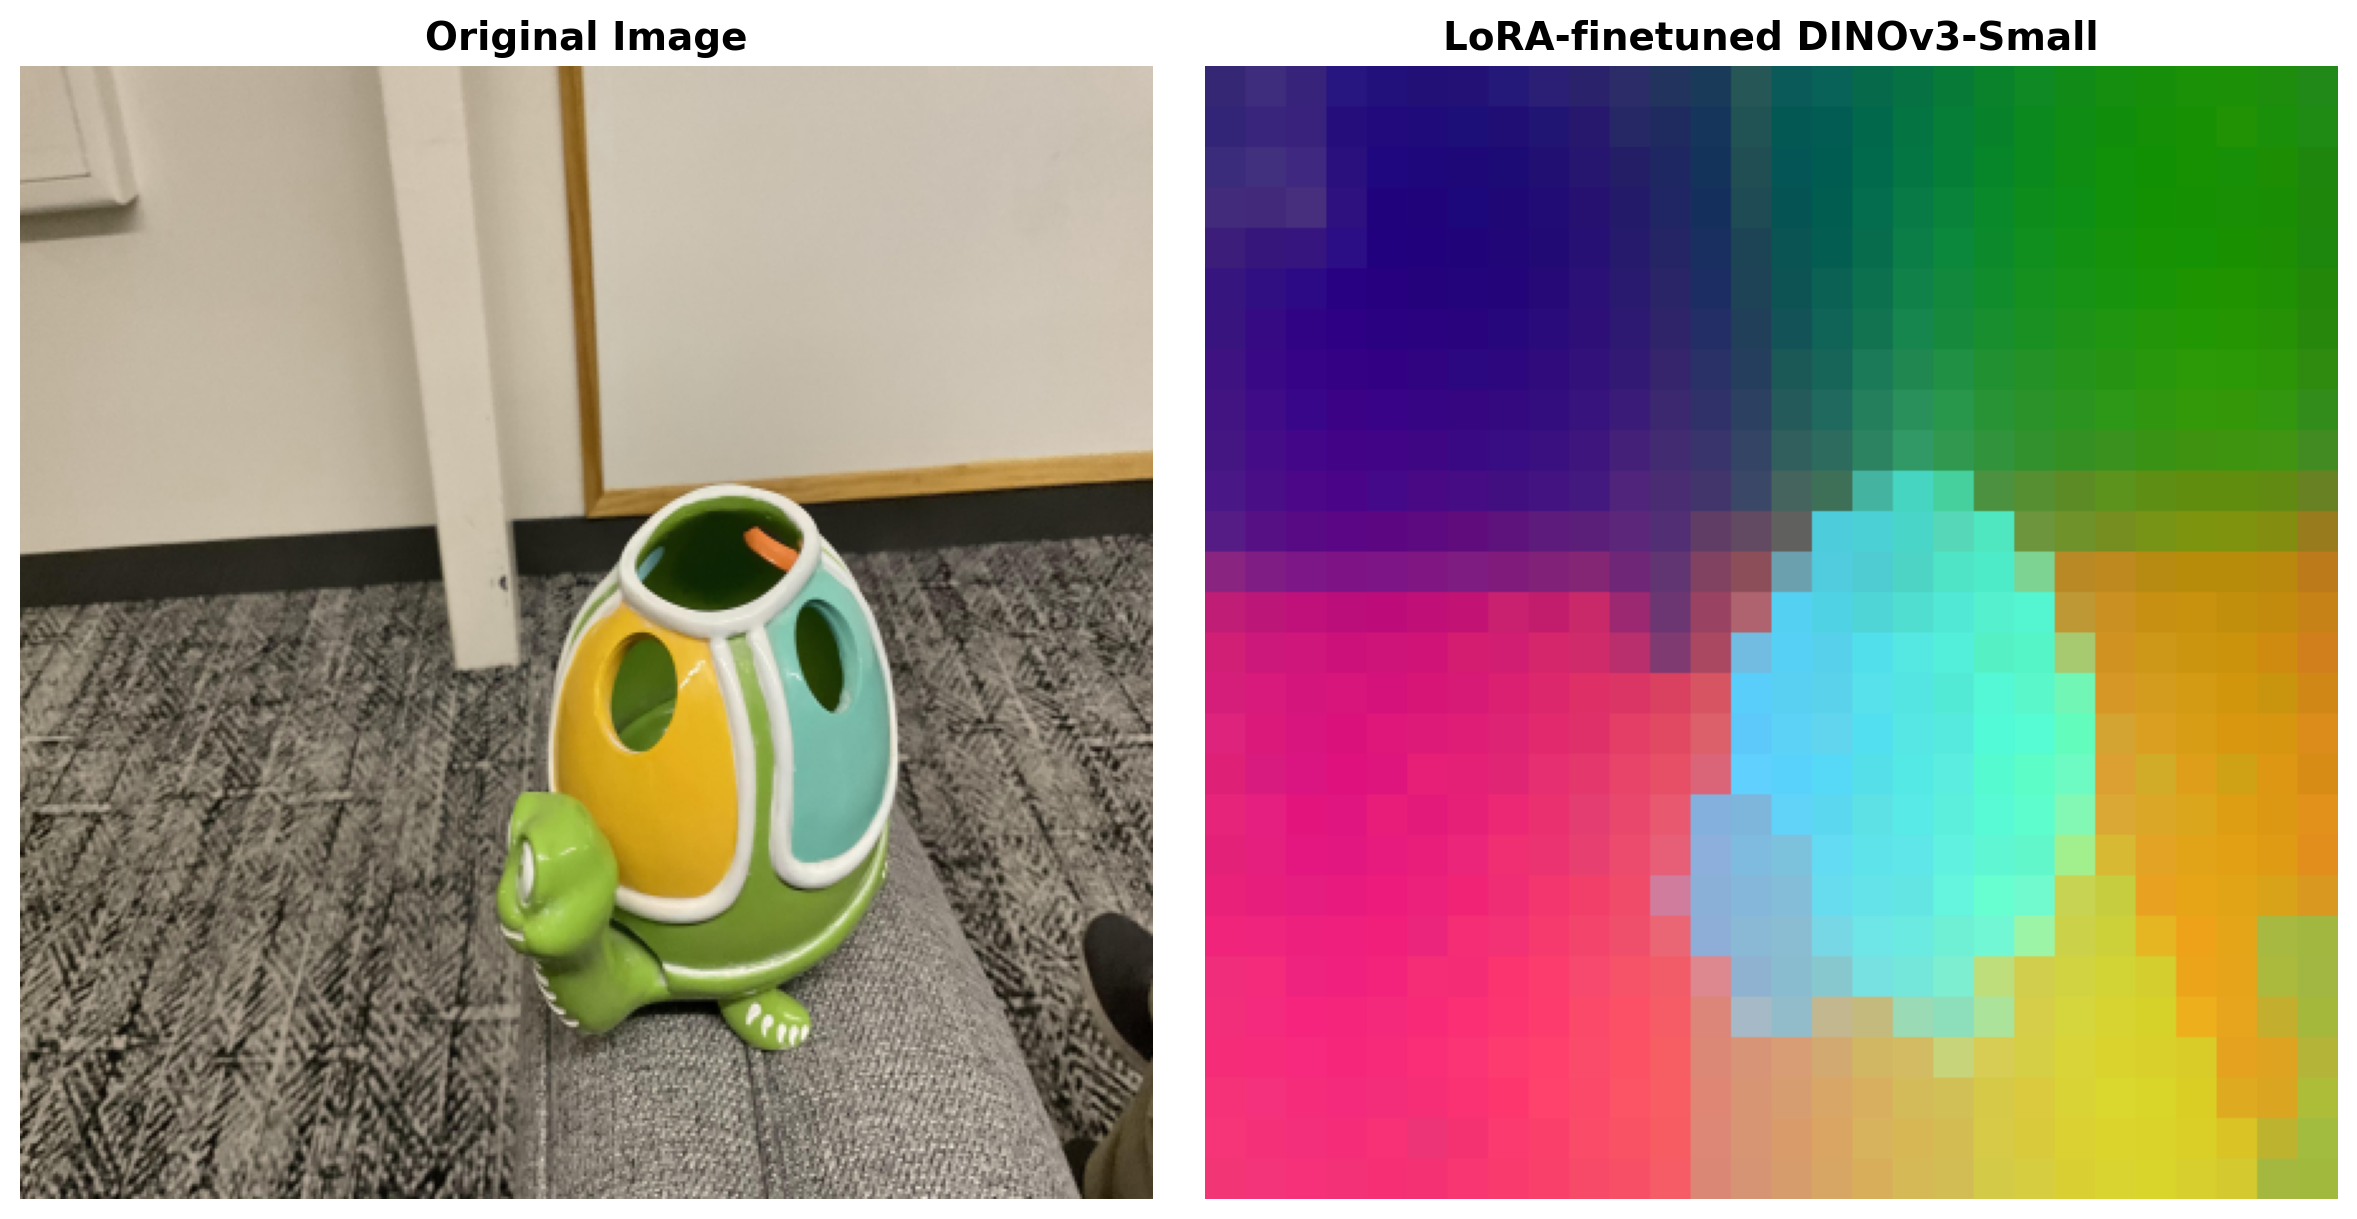
\includegraphics[width=\linewidth]{../presentation/result/diag_small/pca_small_004_lora.png}
\caption{ViT-S/16: LoRA}
\end{subfigure}\\[2pt]
\begin{subfigure}{0.49\linewidth}
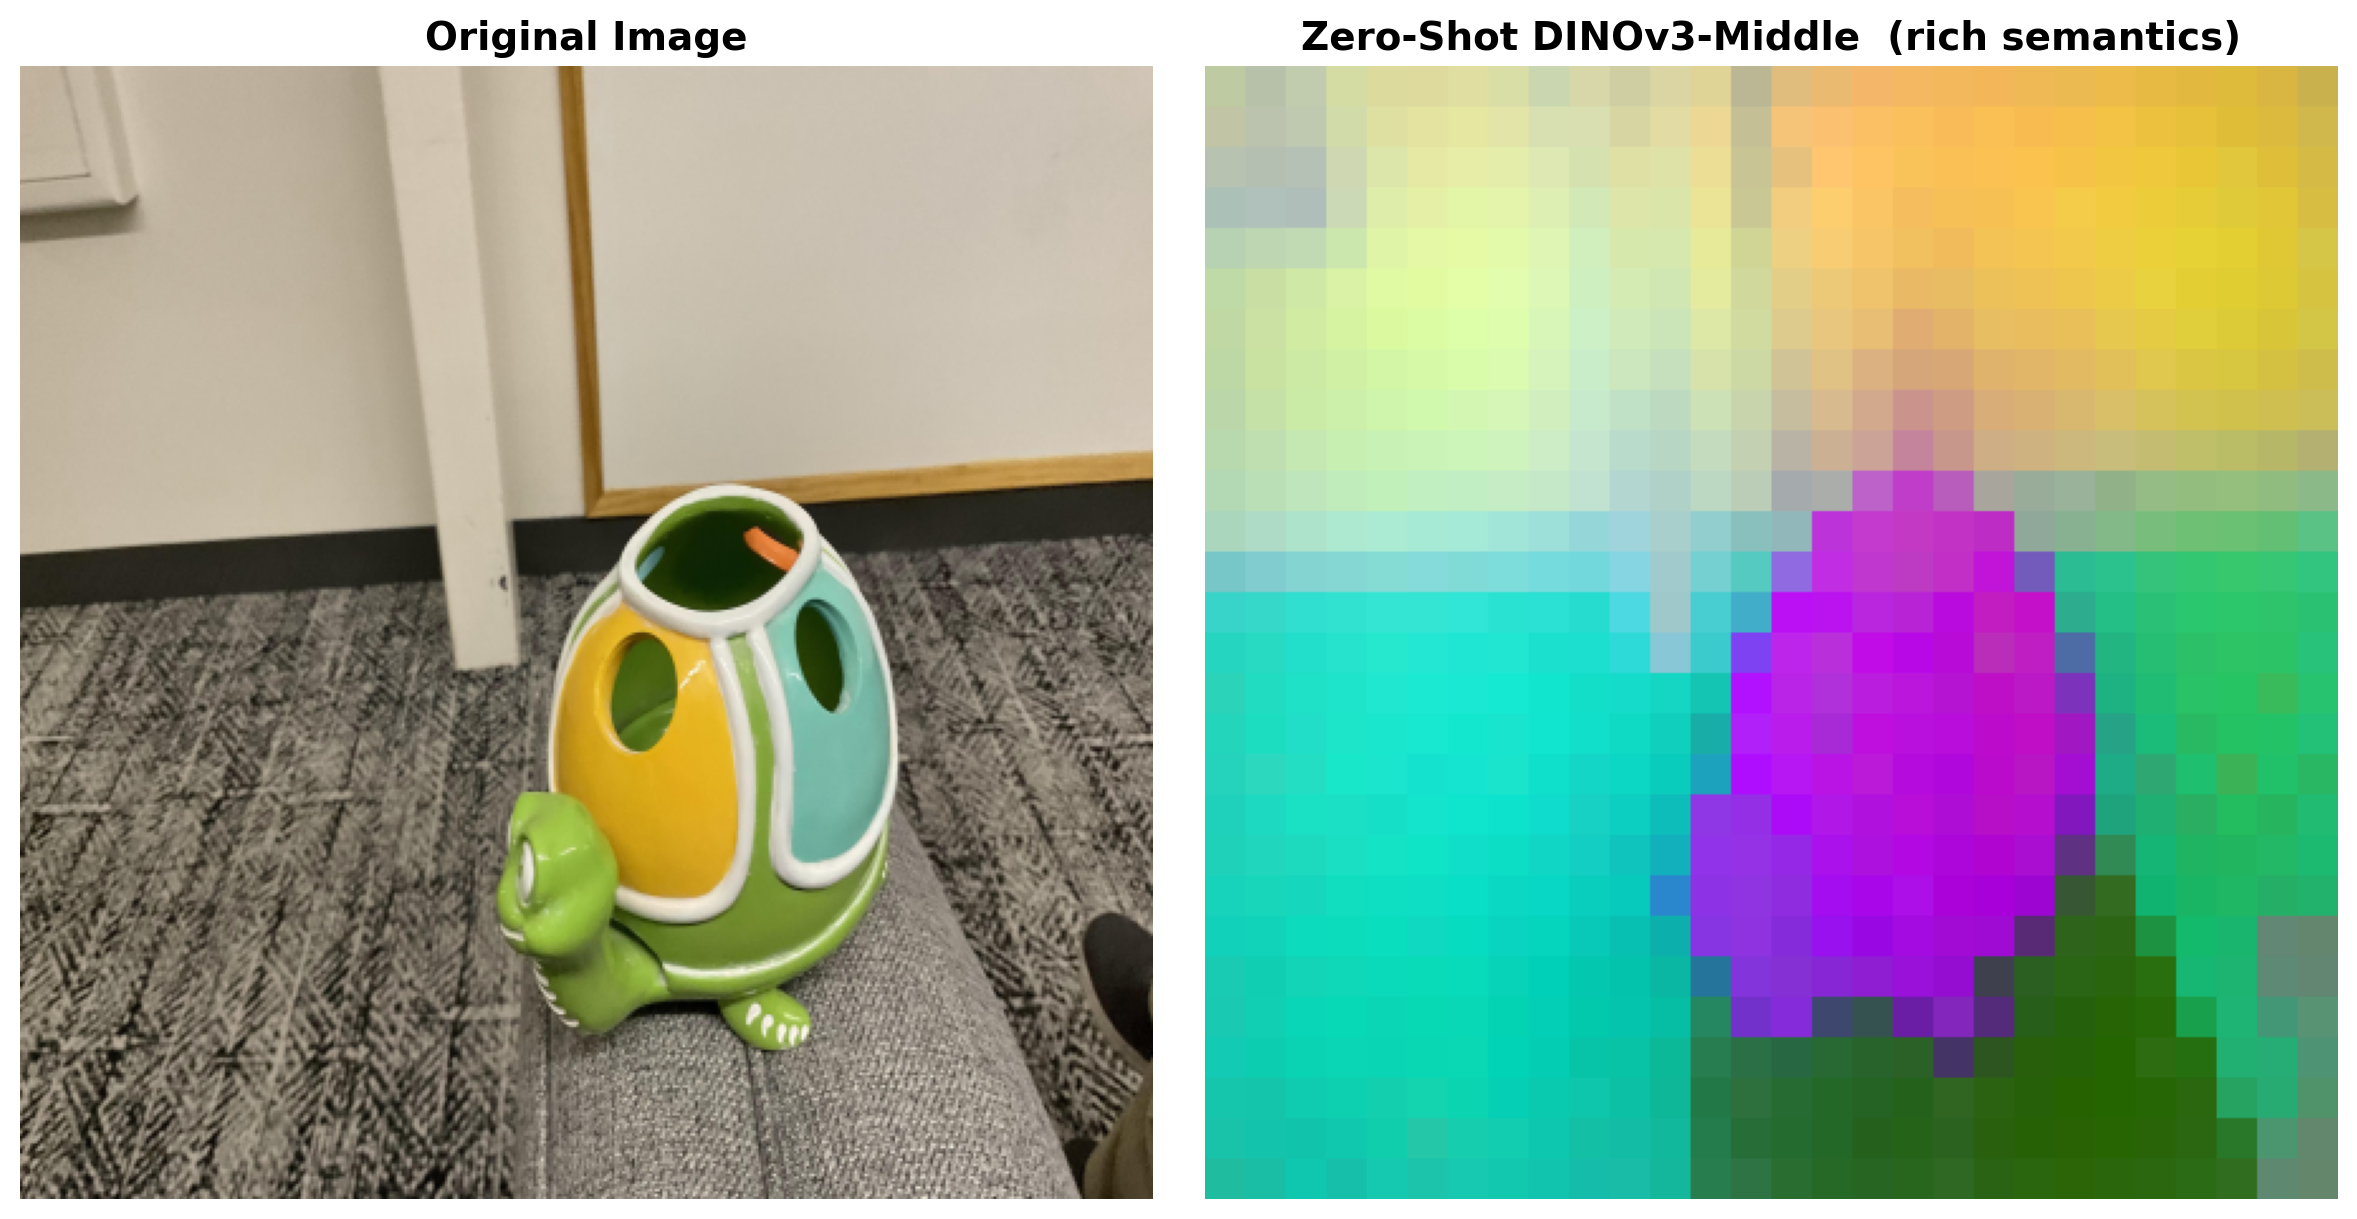
\includegraphics[width=\linewidth]{../presentation/result/diag_middle/pca_middle_004_zs.png}
\caption{ViT-L/16: zero-shot}
\end{subfigure}\hfill
\begin{subfigure}{0.49\linewidth}
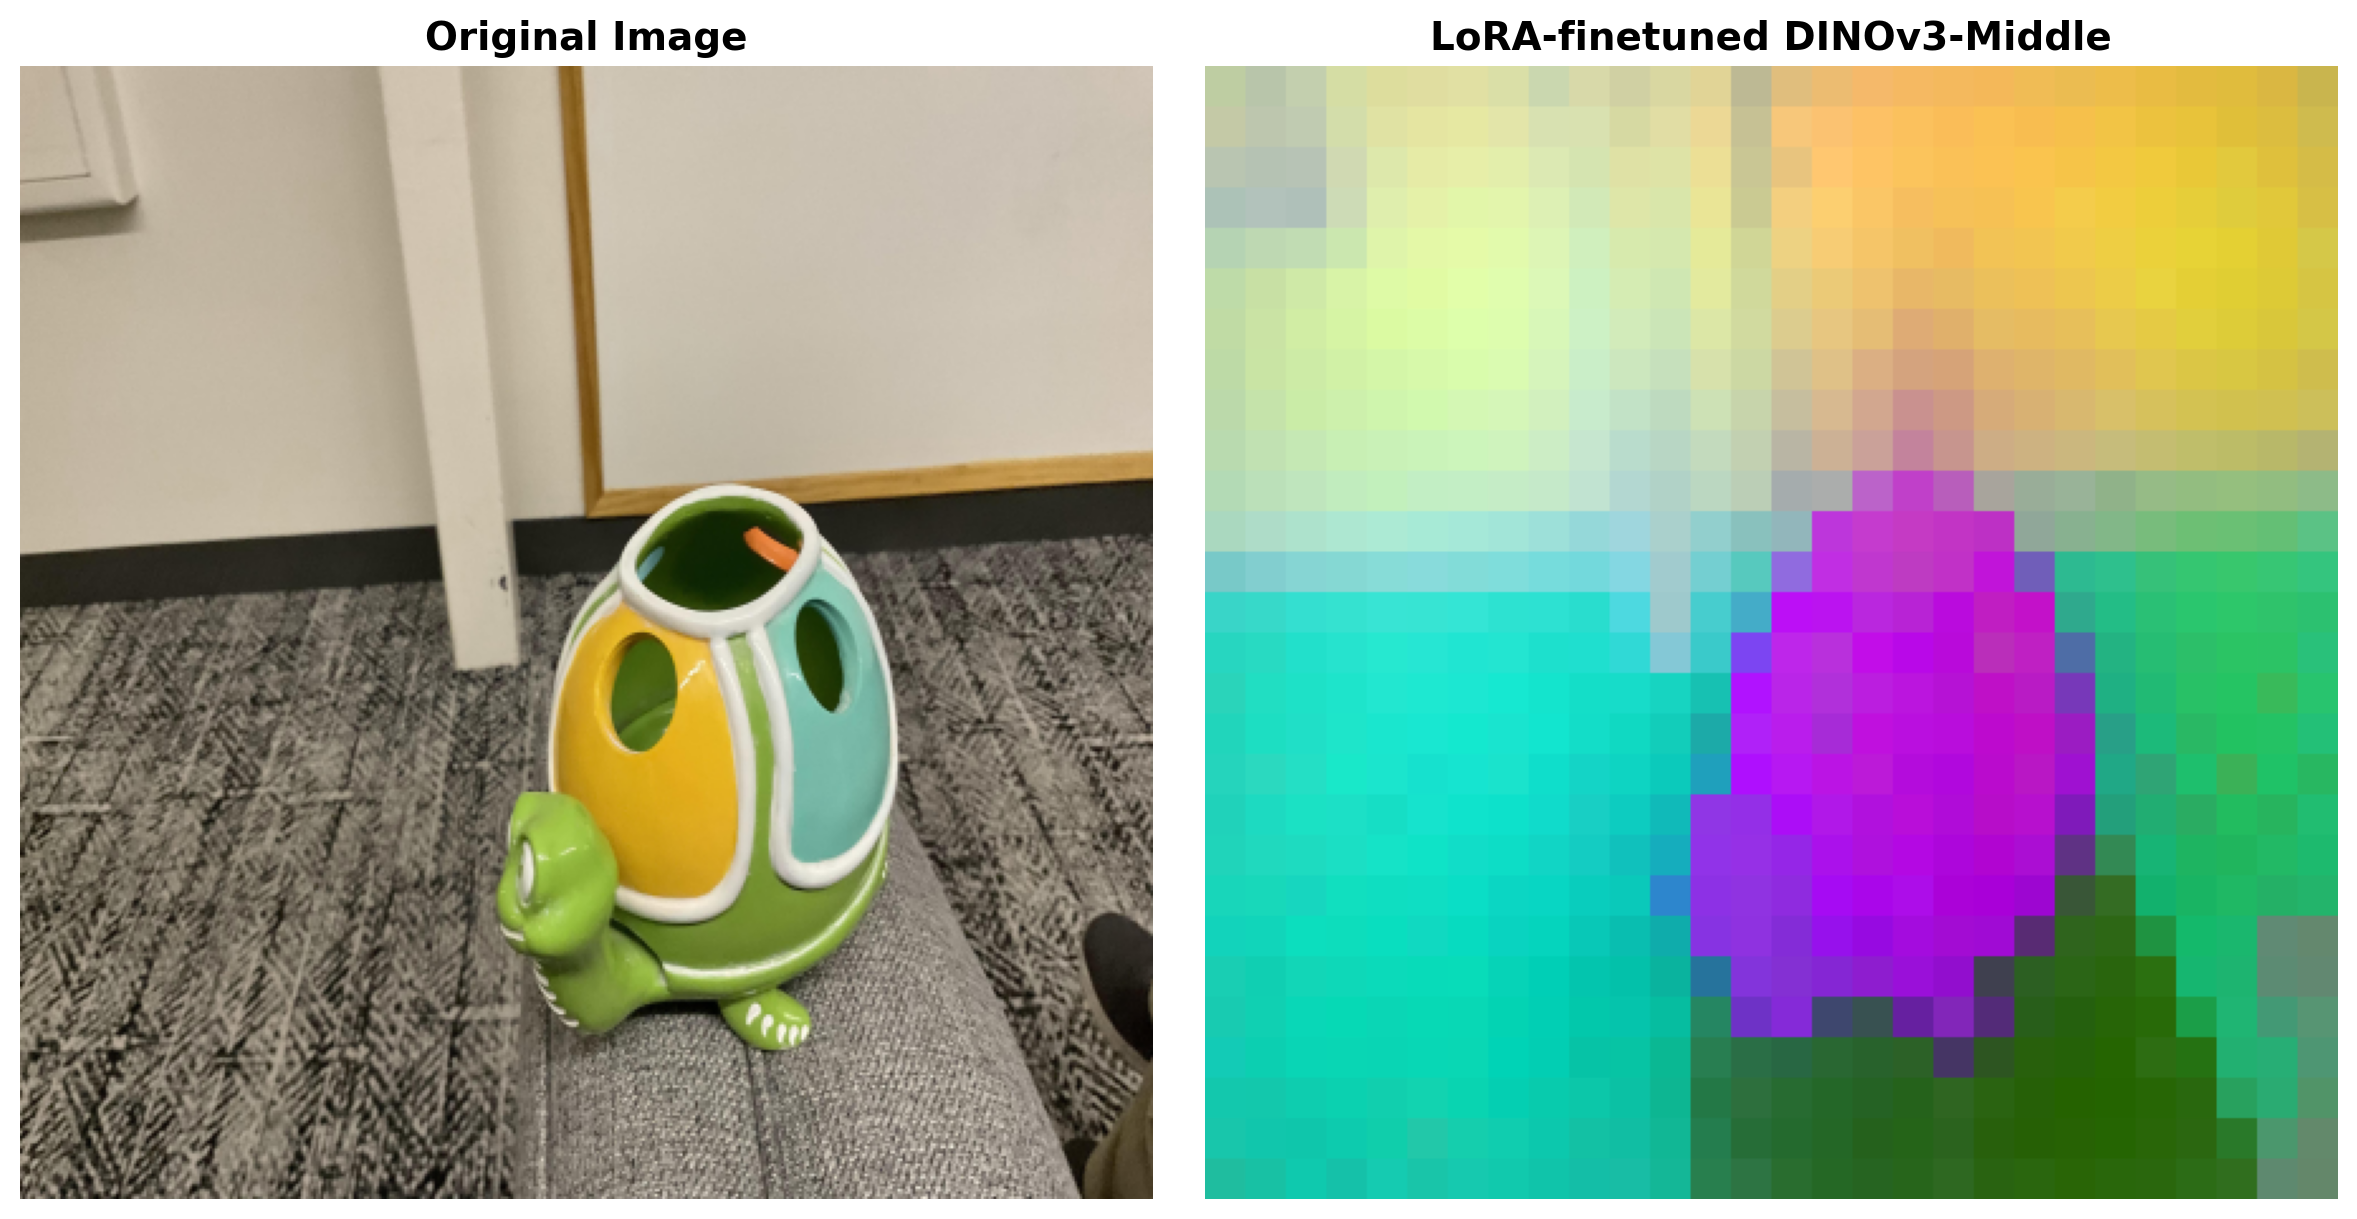
\includegraphics[width=\linewidth]{../presentation/result/diag_middle/pca_middle_004_lora.png}
\caption{ViT-L/16: LoRA}
\end{subfigure}
\caption{PCA-to-RGB visualization of patch tokens, arranged as a
$2\times 2$ grid (rows: backbone size; columns: zero-shot vs.\ LoRA).
The four panels are nearly indistinguishable, supporting the claim
that the LoRA fine-tune does not redraw the feature space.}
\label{fig:pca}
\end{figure}

\paragraph{Layer-4 pose probe (ViT-L/16).} As an additional check we
read out features from an intermediate block (Layer~4) and look at
the relationship between the relative camera-pose angle of a NAVI
pair and the cosine similarity of its mean Layer-4 features
(Fig.~\ref{fig:layer4}). Both the scatter and the per-bin
histograms show only a weak relationship; LoRA fine-tuning does not
make Layer-4 features pose-disentangled.

\begin{figure}[t]
\centering
\begin{subfigure}{0.55\linewidth}
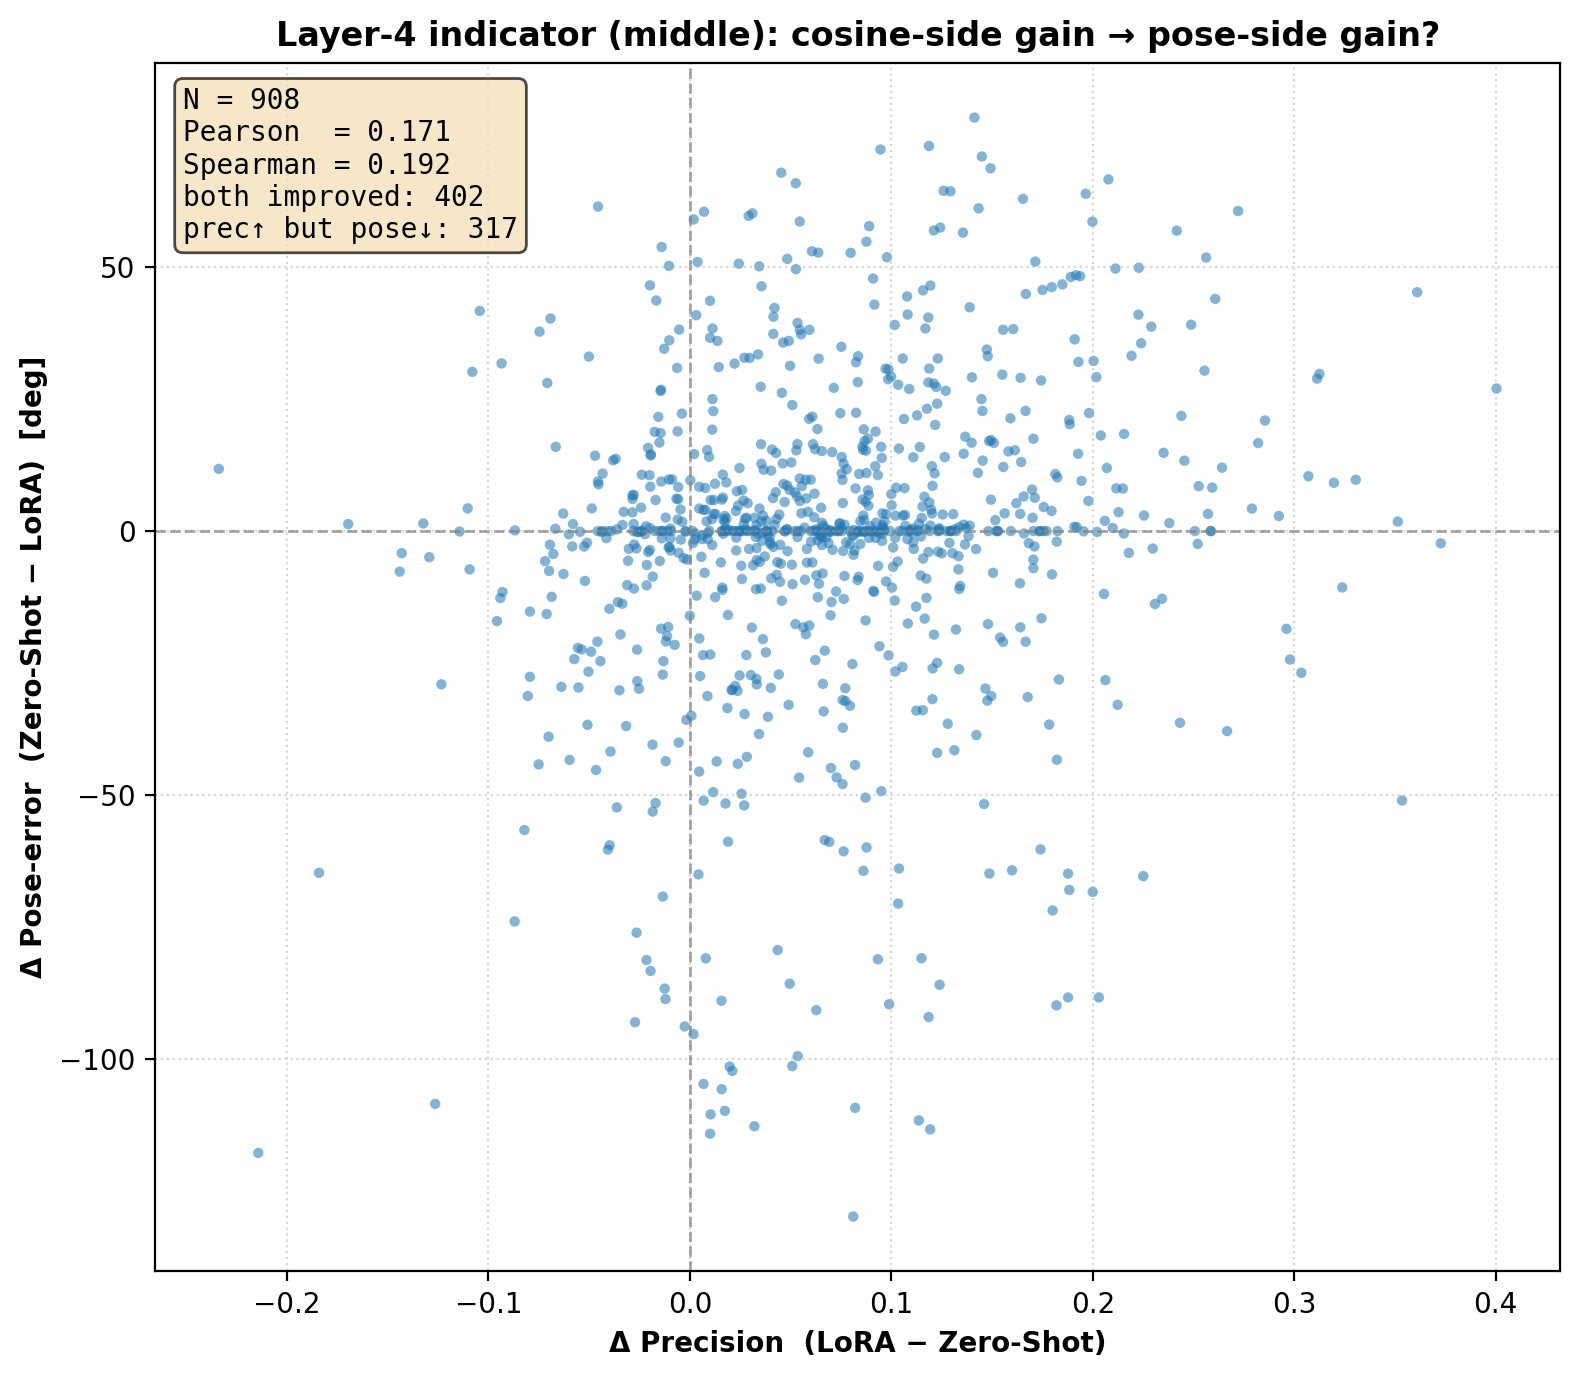
\includegraphics[width=\linewidth]{../presentation/result/diag_middle/layer4_scatter_middle.png}
\caption{Pose vs.\ cos}
\end{subfigure}\hfill
\begin{subfigure}{0.42\linewidth}
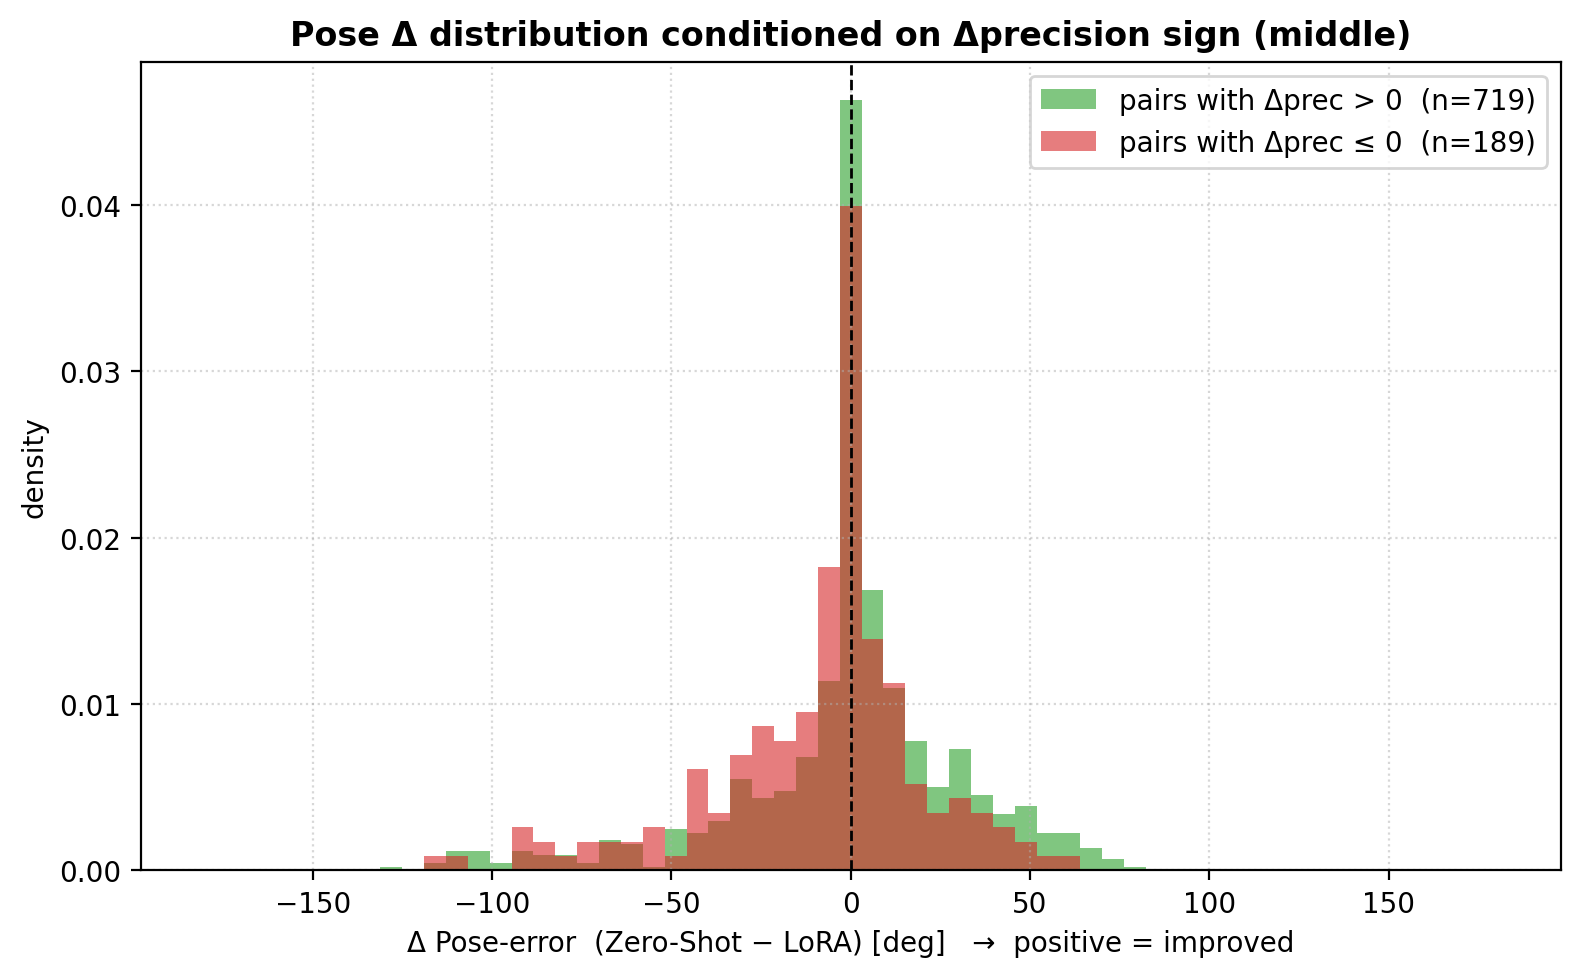
\includegraphics[width=\linewidth]{../presentation/result/diag_middle/layer4_pose_hist_middle.png}
\caption{Bin histogram}
\end{subfigure}
\caption{Layer-4 probe on ViT-L/16. The relationship between
camera-pose angle and intermediate-feature cosine is weak both before
and after fine-tuning, consistent with a small projective tilt rather
than a re-organisation of intermediate representations.}
\label{fig:layer4}
\end{figure}

Taken together, the diagnostics paint a consistent picture: the NAVI
matching gain is real and reproducible, but it does \emph{not}
originate from a redesigned feature space. LoRA introduces a small,
low-rank rotation of the existing DINOv3 features that happens to be
aligned with NAVI's matching decision boundary; the underlying
representation is essentially unchanged.

\section{Limitations and Discussion}
\label{sec:limits}

We summarise the shortcomings so that they are not misread as
features. (i) \emph{Strict-threshold pose accuracy does not improve}:
AUC@$5^\circ$ is $0.000$ for the best ViT-S/16 model and within noise
for ViT-L/16. The recipe trades strictly correct poses for
loosely-correct poses; downstream applications requiring few-degree
accuracy do not yet benefit. (ii) \emph{The feature space barely
moves}: intra-image cosine, positive-pair cosine, effective rank,
neighbourhood dominance and PCA visualizations all change by
$\le 0.02$. (iii) \emph{Layer-wise behaviour is not pose-disentangled}.
(iv) \emph{NAVI is single-object}; whether gains generalise to
MegaDepth, ScanNet or IMC-2021 is untested. (v) \emph{No comparison to
specialised matchers}: our scope is bounded to ``zero-shot DINOv3
vs.\ LoRA-tuned DINOv3''.

The corresponding strengths are: (1) zero-init LoRA means the
contrastive loss can only \emph{add} information; (2) cross-scene
negatives at $B=8$ avoid the trivial $\ln(K\!+\!1)$ floor; (3) the
5-patch Safe-Radius mask removes the in-image negatives that would
otherwise fight DINOv3's smoothness prior. The two backbones behave
qualitatively the same: per-epoch curves are smooth and final gains
are within one percentage point of each other (Precision $+7.7$ pp
on S/16, $+7.0$ pp on L/16). The smaller absolute Precision of L/16
at zero-shot ($16.8\%$ vs.\ $17.4\%$) is a known artefact of the
higher feature dimensionality interacting with NAVI's evaluation
geometry; the fine-tuned models close this gap on AUC@$20^\circ$ in
favour of L/16 ($1.123$ vs.\ $1.040$).

\section{Conclusion}

We presented a parameter-efficient fine-tuning recipe for DINOv3
dense features that is small in code (LoRA on Q/V, HardInfoNCE,
5-patch Safe-Radius mask), small in trainable parameters (rank-4
adapters), and small in compute (15 epochs on NAVI). On both
ViT-S/16 and ViT-L/16 it improves NAVI matching Precision by
roughly $+7$ pp and more than doubles AUC@$20^\circ$ over the
zero-shot baseline, with stable per-epoch behaviour. At the same
time, the diagnostic analysis and the explicit limitations list
make clear what this recipe is \emph{not}: it does not reshape the
DINOv3 feature space, it does not improve strict-threshold pose
accuracy, and it has only been validated on a single-object dataset.
The honest reading is therefore that LoRA + HardInfoNCE + Safe Radius
applies a \emph{small low-rank tilt} to frozen DINOv3 features that
is well-aligned with NAVI's matching decision boundary, but is far
from a full geometric fine-tune. Closing the AUC@$5^\circ$ gap
plausibly requires either training on multi-scene data with explicit
hard-negative mining across scenes, or a stronger adapter family
(e.g.\ joint LoRA on Q/K/V plus the FFN), both of which we leave to
future work.

\section*{Author Contributions}

The four team members contributed equally to this project, with a
workload distribution of $25\%$ each (totalling $100\%$).

\textbf{Dai Xunlian (225040015, 25\%)} co-designed the overall
recipe (LoRA on Q/V, HardInfoNCE, Safe Radius), implemented the
LoRA injection module and the training loop, ran the ViT-S/16 and
ViT-L/16 fine-tuning experiments, and co-drafted the Method and
Experiments sections.

\textbf{Mu Ruotong (225040014, 25\%)} built the NAVI data pipeline
(scene-disjoint split, depth-based positive correspondence
generation, training/test pair construction), implemented the
HardInfoNCE loss and the 5-patch Safe-Radius mask, produced the
per-epoch evaluation curves, and co-drafted the Dataset and
Protocol subsections.

\textbf{Li Langye (225040134, 25\%)} implemented the diagnostic
analysis (intra-image / positive-pair cosine, effective rank,
neighbourhood dominance, PCA-to-RGB visualization, Layer-4 pose
probe), produced all diagnostic figures, and co-drafted the
Diagnostic Analysis subsection together with the Limitations
discussion.

\textbf{Li Mingzhe (225045024, 25\%)} implemented the
SuperGlue-style pose-evaluation pipeline (MNN, USAC, 5-pt with
cheirality, AUC@$5/10/20$ and Precision metrics), managed the
HuggingFace \texttt{Dinov3ViTModel} integration and the
reproducibility scripts, and co-drafted the Introduction, Related
Work and Conclusion sections.

All four authors jointly discussed the design decisions, reviewed
each other's writing, and agree on the final version of the
report.
{
    \small
    \bibliographystyle{ieeenat_fullname}
    \bibliography{../references}
}

\end{document}
